\documentclass[11pt,a4paper]{article}
\usepackage[margin=25mm]{geometry}
\usepackage{amsmath,amssymb}
\usepackage{graphicx}
\usepackage{hyperref}
\usepackage{booktabs}

\title{Machine Learning-based Prediction of Elastic Modulus in High-Entropy and Multi-Principal Element Alloys}
\author{AI\_metallurgy Project Team}
\date{2026-01-23}

\begin{document}

\maketitle

\begin{abstract}
The elastic modulus mismatch between metallic implants and human bone is a long-standing challenge in biomedical materials design. High-entropy alloys (HEAs) and multi-principal element alloys (MPEAs) offer great compositional flexibility for tuning mechanical properties, but systematic exploration of the vast composition space is experimentally expensive. In this work, we compile and integrate elastic modulus data from multiple experimental and computational sources and develop machine-learning models to predict the elastic modulus of HEA/MPEA systems. The integrated dataset contains 5{,}339 alloys (approximately 6.3\% experimental and 93.7\% computed) after cleaning and de-duplication, with Young's modulus values spanning from about 2.7~GPa to 621~GPa. We construct 29 physically motivated features including composition descriptors (e.g., Ti, Zr, Nb fractions), atomic descriptors (atomic radius, electronegativity, valence electron concentration), and density-related quantities. Using this feature set, we benchmark linear and non-linear regression models, including linear and regularized regressions, tree-based ensembles, support vector regression (SVR), gradient boosting, and a feedforward neural network. An optimized SVR model achieves a test coefficient of determination of $R^2 \approx 0.59$ on a 322-sample dataset, while a gradient boosting model attains $R^2 \approx 0.67$ on an experimental-only subset, demonstrating practically useful predictive capability. Feature-importance analyses consistently highlight Ti content, average electronegativity, valence electron concentration, and density as key drivers of the elastic modulus. We discuss the implications for designing low-modulus HEAs for biomedical implants, limitations arising from mixed experimental and computational data, and directions for extending the models and dataset.
\end{abstract}

\section{Introduction}

Metallic implants such as hip and knee replacements must satisfy demanding mechanical and biological requirements. A particularly important issue is the elastic modulus mismatch between conventional metallic biomaterials (e.g., Ti--6Al--4V, Co--Cr alloys, stainless steels) and cortical bone. Human bone typically exhibits Young's modulus values in the range of roughly 10--30~GPa, while common metallic implant alloys often have moduli in the range of 100--200~GPa or higher. This mismatch can lead to stress shielding, bone resorption, and long-term implant loosening.

High-entropy alloys (HEAs) and multi-principal element alloys (MPEAs) have emerged as promising candidates for next-generation structural and functional materials. Their compositional flexibility enables tailoring of properties such as strength, ductility, corrosion resistance, and elastic modulus. In the biomedical context, HEAs based on biocompatible elements (e.g., Ti, Zr, Nb, Ta, Hf) offer the possibility of achieving reduced stiffness while maintaining adequate strength and corrosion resistance. However, the design space spanned by multi-component compositions and processing conditions is enormous, making exhaustive experimental exploration infeasible.

Several databases and studies have documented mechanical properties of HEAs and related alloys. The database by Gorsse \textit{et al.} compiles mechanical properties for HEAs and complex concentrated alloys, including Young's modulus for a large set of alloys. A DOE/OSTI dataset provides experimental Young's modulus values and related descriptors for high-entropy alloys. Large-scale computational databases such as the Materials Project publish density-functional-theory (DFT) elastic tensors for inorganic compounds, from which bulk, shear, and Young's moduli can be derived. Additional datasets, such as MPEA mechanical-property compilations and nano-indentation databases, further expand the available information.

The AI\_metallurgy project leverages these resources to build an integrated, cleaned dataset of HEA/MPEA elastic modulus values and to train machine-learning models that can predict the modulus from composition and derived descriptors. Earlier phases of the project focused on an experimentally dominated subset of 322 alloys, for which multiple regression models were developed and optimized. In this report, we consolidate the full data pipeline and modeling results into a single narrative suitable for scientific manuscripts or extended technical documentation.

\begin{figure}[htbp]
\centering
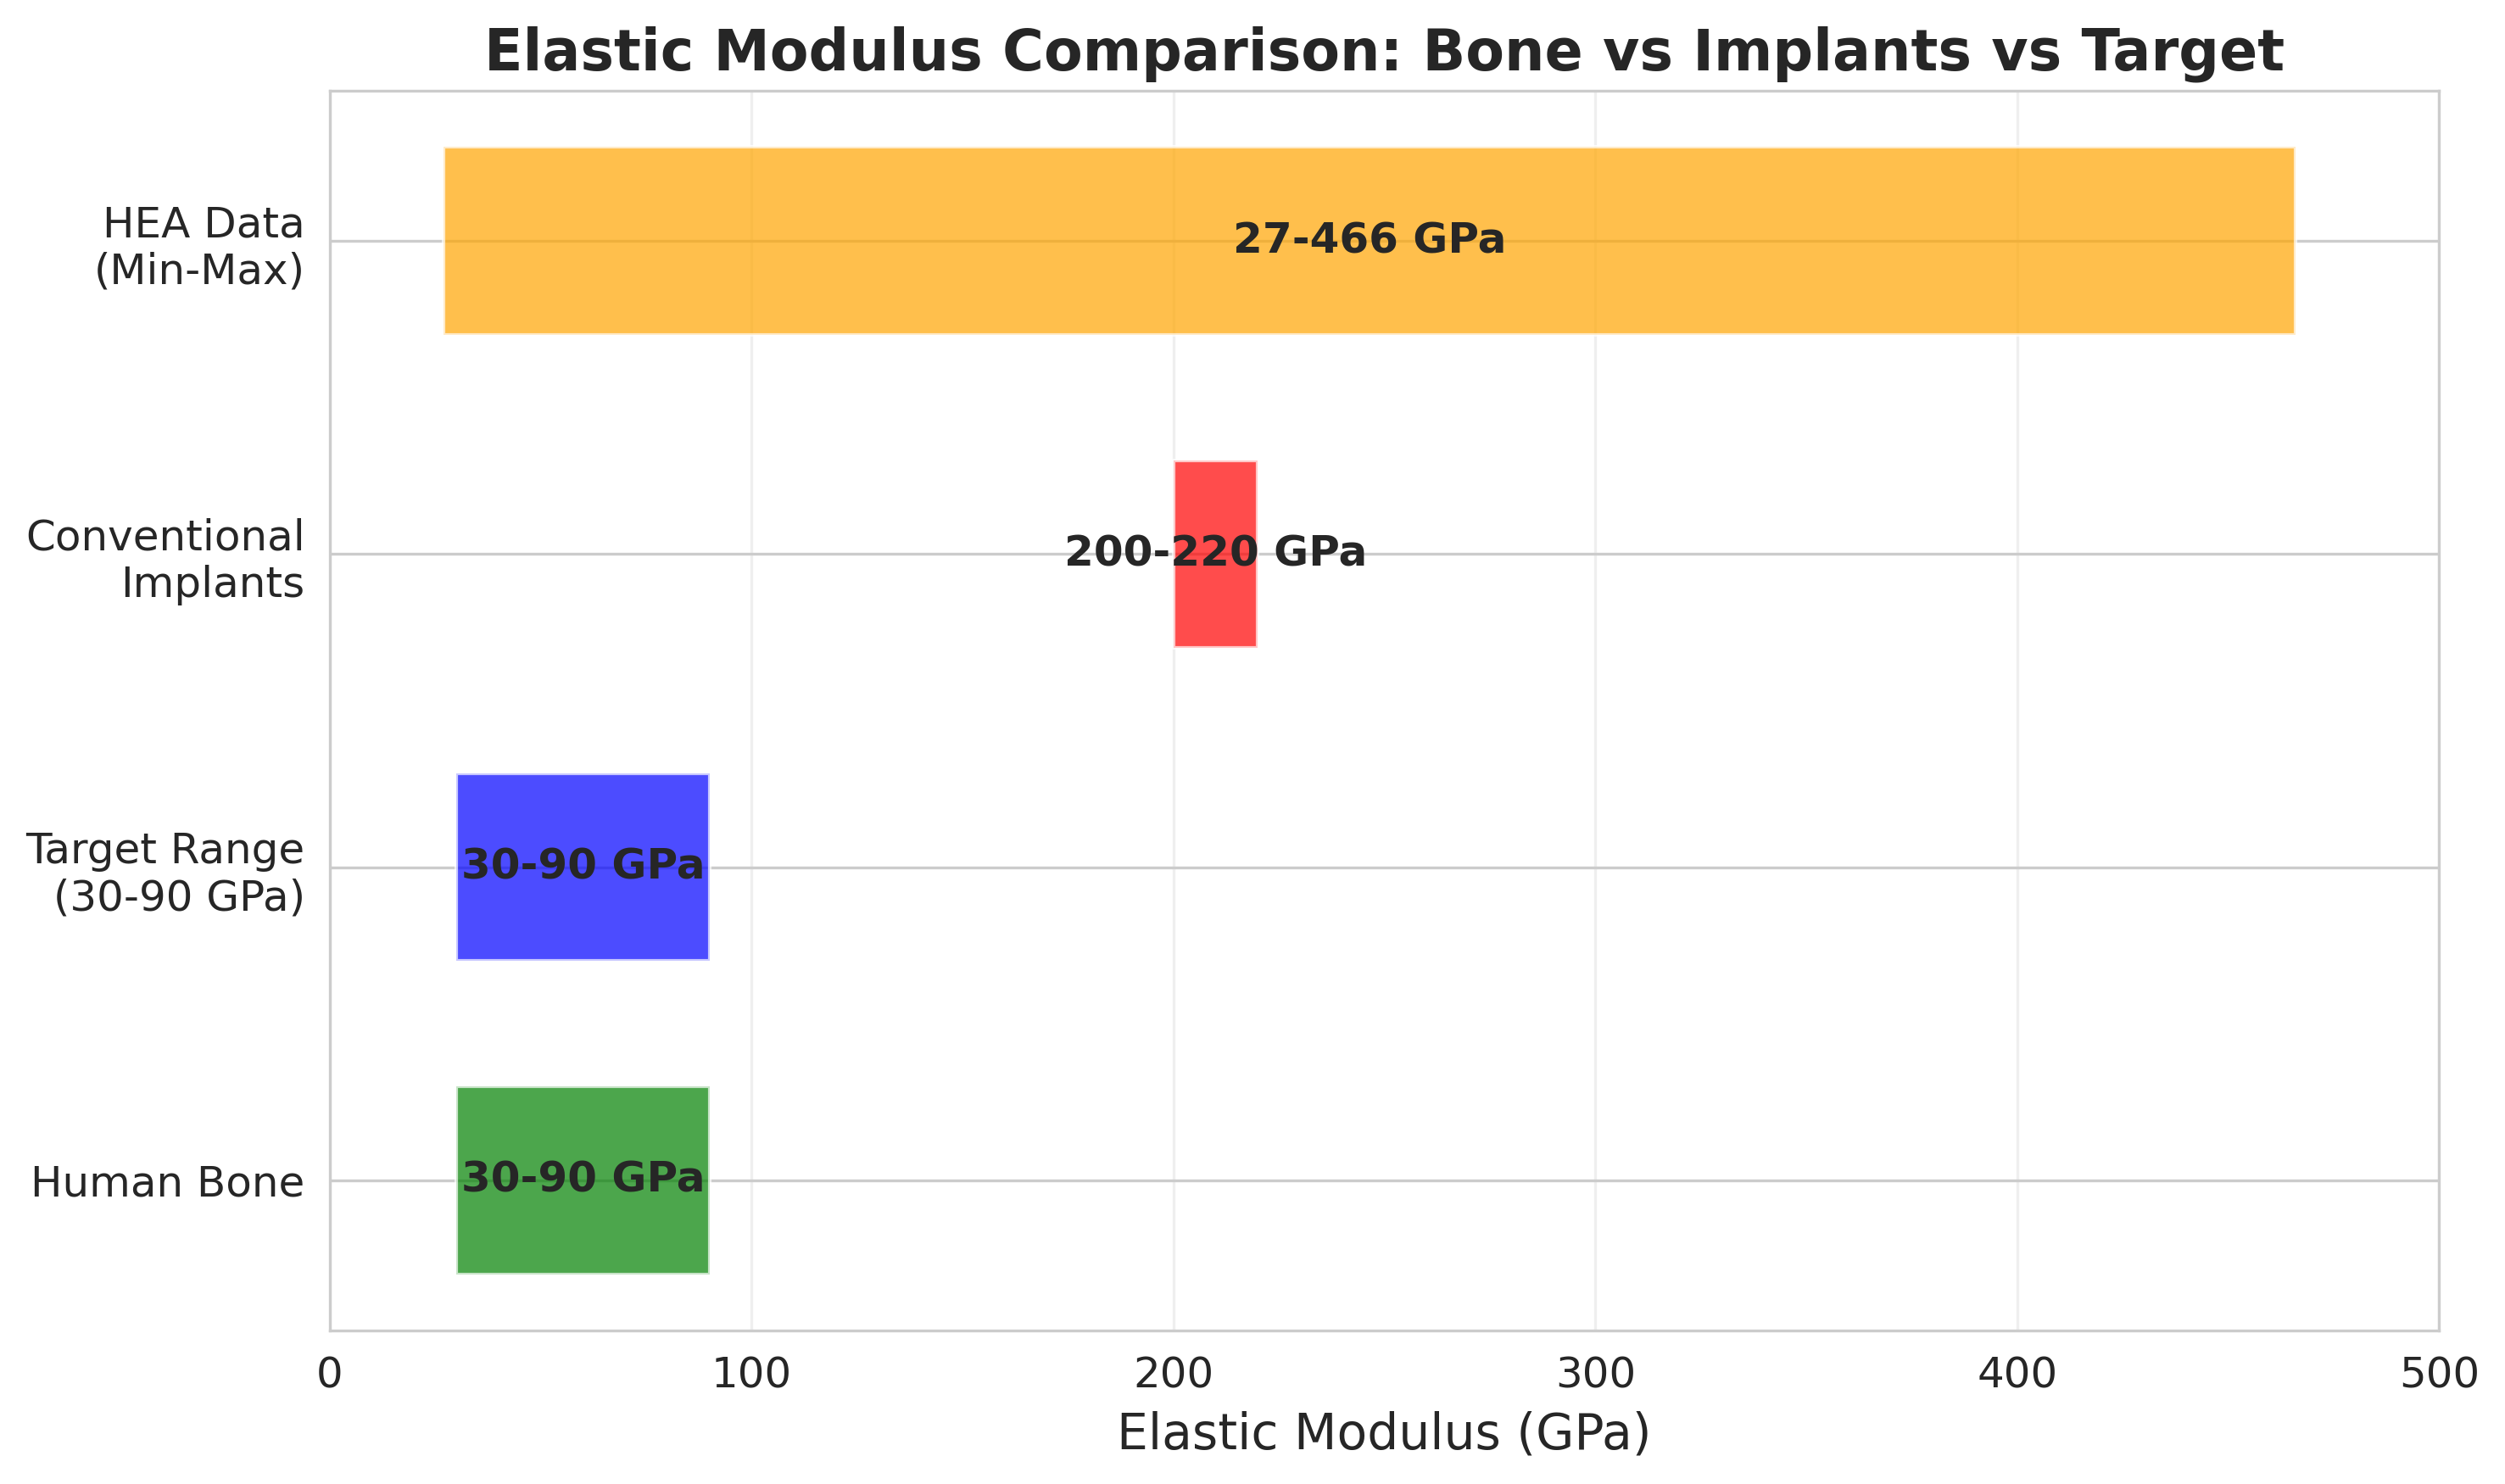
\includegraphics[width=0.85\textwidth]{figures/elastic_modulus_comparison.png}
\caption{Comparison of elastic modulus ranges for human bone, conventional metallic biomaterials, and target range for biomedical HEA/MPEA alloys. The mismatch between bone (10--30~GPa) and traditional implants (100--200~GPa) motivates the design of low-modulus alloys in the 30--90~GPa range.}
\label{fig:elastic_modulus_comparison}
\end{figure}

\section{Data and Dataset Construction}

\subsection{Data Sources}

The final integrated dataset is constructed from a combination of experimental and computational sources:

\begin{itemize}
  \item \textbf{DOE/OSTI HEA dataset (experimental)}: A curated dataset of high-entropy alloys with phase information and experimentally measured Young's modulus for a subset of alloys. After de-duplication and cleaning, 101 alloys with valid modulus values are retained.
  \item \textbf{Gorsse HEA mechanical-properties database (experimental)}: A literature-based database of HEAs and complex concentrated alloys with composition, microstructure, density, hardness, strength, elongation, and Young's modulus. We include 182 unique alloys with valid Young's modulus.
  \item \textbf{Latest experimental HEA data}: Additional data from recent publications on Ti--Zr--Nb, Ti--Zr--Hf--Nb--Ta, and related biocompatible HEA/MPEA systems. Due to overlaps with earlier databases and nano-indentation compilations, the net increase in unique alloys is modest.
  \item \textbf{MPEA nano-indentation dataset (experimental and computed)}: A dataset of phase-specific mechanical properties measured by nano-indentation in multi-principal element alloys. From this dataset, we extract 51 experimental entries and 196 calculated entries with Young's modulus after integration.
  \item \textbf{Refractory HEA elastic-constants dataset (computed)}: A set of DFT-computed elastic constants for 370 refractory HEAs, from which Young's modulus is derived.
  \item \textbf{Materials Project (computed)}: DFT-derived elastic tensors for a large number of inorganic compounds. For suitable compositions related to HEA/MPEA chemistries, Young's modulus is computed via
  \begin{equation}
    E = \frac{9KG}{3K + G},
  \end{equation}
  where $K$ and $G$ are bulk and shear moduli, respectively. This source contributes 4{,}439 samples.
\end{itemize}

Auxiliary databases such as DISMA and MPEA mechanical-property compilations are used for cross-checking and metadata but are not primary sources for the target property.

\subsection{Integration and Cleaning}

Each dataset is first parsed into a standardized tabular format with at least an alloy identifier, Young's modulus in GPa, and a source label. The main integration steps are:

\begin{enumerate}
  \item Column harmonization to a unified label \texttt{elastic\_modulus} in GPa;
  \item Removal of entries with missing, non-positive, or clearly unphysical modulus values;
  \item Duplicate detection and removal based on alloy name, composition, and modulus;
  \item Enforcement of mandatory fields (\texttt{alloy\_name}, \texttt{elastic\_modulus}, \texttt{source});
  \item Validation of the final table using dedicated scripts that check schema consistency, missing values, duplicates, and basic statistics.
\end{enumerate}

The final cleaned dataset is stored as \texttt{unified\_dataset\_cleaned\_20260123\_175245.csv} (with a stable copy \texttt{unified\_dataset\_latest.csv}) and contains 5{,}339 unique alloy entries.

\subsection{Dataset Characteristics}

The 5{,}339-sample integrated dataset has the following key attributes:

\begin{itemize}
  \item Source breakdown:
    \begin{itemize}
      \item Materials Project: 4{,}439 samples (83.1\%);
      \item Refractory HEA elastic constants: 370 samples (6.9\%);
      \item MPEA nano-indentation (calculated): 196 samples (3.7\%);
      \item Gorsse database: 182 samples (3.4\%);
      \item DOE/OSTI: 101 samples (1.9\%);
      \item MPEA nano-indentation (experimental): 51 samples (1.0\%).
    \end{itemize}
  \item Experimental vs.\ computed:
    \begin{itemize}
      \item Experimental Young's modulus: 335 samples ($\approx 6.3$\%);
      \item Computed Young's modulus: 5{,}004 samples ($\approx 93.7$\%).
    \end{itemize}
  \item Young's modulus distribution:
    \begin{itemize}
      \item Minimum: 2.73~GPa;
      \item Maximum: 621.33~GPa;
      \item Mean: 139.26~GPa;
      \item Median: 122.61~GPa.
    \end{itemize}
\end{itemize}

An earlier phase of the project used a predominantly experimental subset of 322 alloys (from DOE/OSTI, Gorsse, and recent experiments) for model development. In that subset, Young's modulus ranges approximately from 27--466~GPa, with about 30 alloys in the 30--90~GPa range relevant for bone-like stiffness.

\begin{figure}[htbp]
\centering
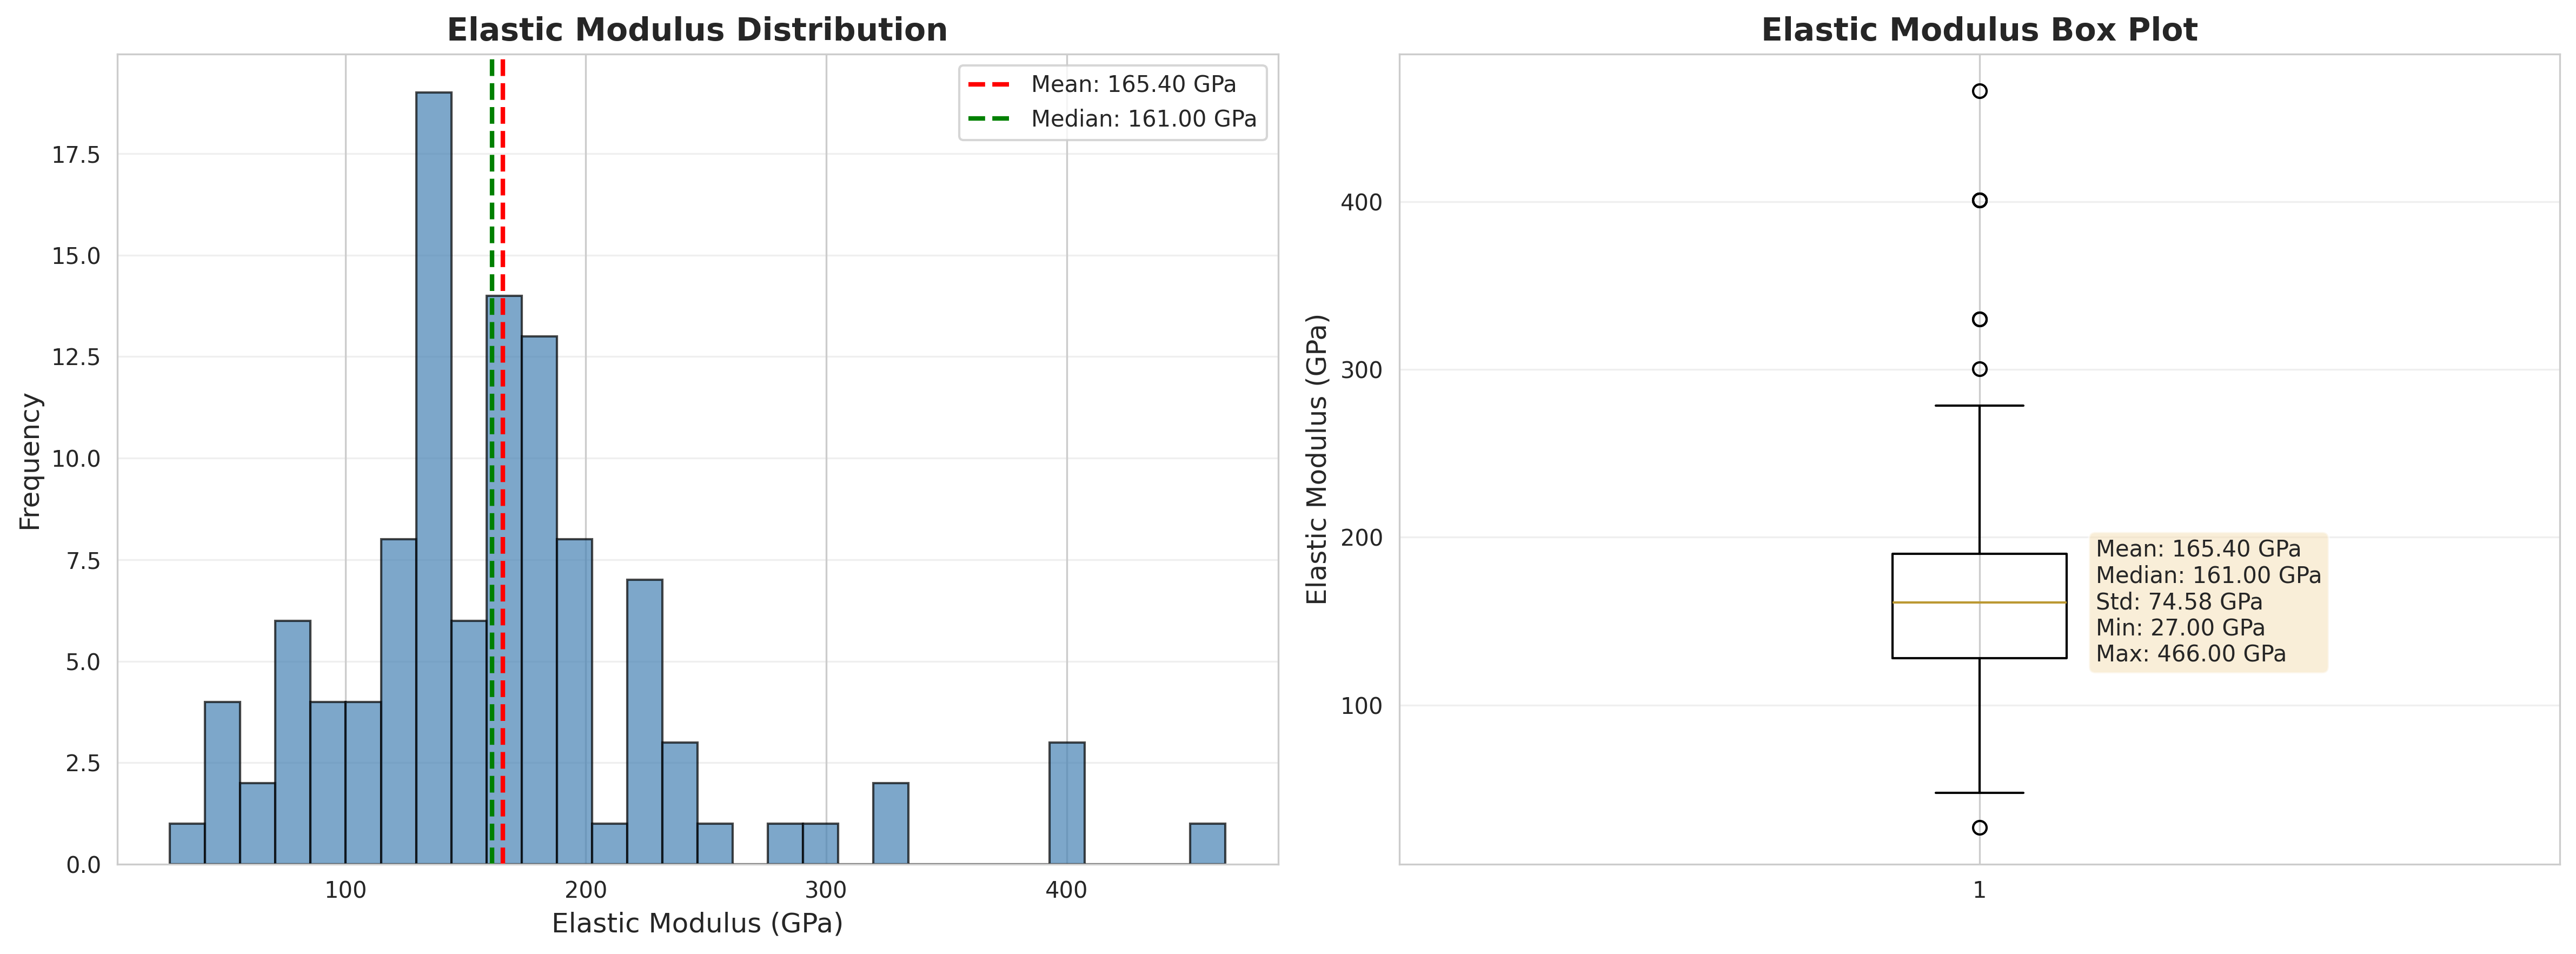
\includegraphics[width=0.85\textwidth]{figures/data_distribution.png}
\caption{Distribution of elastic modulus values in the integrated dataset (5{,}339 samples). The histogram shows a broad distribution spanning from approximately 2.7~GPa to 621~GPa, with a mean around 139~GPa. The target range for biomedical applications (30--90~GPa) is highlighted.}
\label{fig:data_distribution}
\end{figure}

\begin{figure}[htbp]
\centering

\includegraphics[width=0.85\textwidth]{figures/data_characteristics.png}
\caption{Key characteristics of the integrated dataset, including source breakdown, experimental vs.\ computed data distribution, and statistical properties of the elastic modulus values.}
\label{fig:data_characteristics}
\end{figure}

\section{Features and Machine Learning Methods}

\subsection{Feature Engineering}

We construct 29 features combining composition information with atomic and thermodynamic descriptors. The main categories are:

\begin{itemize}
  \item Atomic-radius descriptors: average, standard deviation, maximum, minimum, and spread of atomic radius;
  \item Electronegativity descriptors: average, standard deviation, and spread of electronegativity;
  \item Electronic/thermodynamic descriptors: valence electron concentration (VEC), configurational mixing entropy, and number of elements;
  \item Composition fractions for 17 elements: Ti, Zr, Hf, Nb, Ta, V, Cr, Mo, W, Fe, Co, Ni, Cu, Al, Mn, Si, Sn;
  \item Additional physical descriptors: density and selected dataset-specific quantities.
\end{itemize}

\subsection{Models and Training Protocol}

We benchmark linear models (linear, Ridge, Lasso), polynomial regression, K-nearest neighbors, tree-based ensemble methods (random forest, gradient boosting, stacking), support vector regression (SVR), and a feedforward neural network. In the broader AI\_metallurgy project, we also implement a family of advanced operator-learning and graph-based models, including Fourier Neural Operators (FNO1d/FNO2d), DeepONet, materials graph networks such as MEGNet and CGCNN, Neural ODEs, physics-informed neural networks (PINNs), graph neural networks (HEAGNN), and a composition-based Transformer (HEATransformer). These architectures are implemented and trained in the \texttt{fno\_models} and \texttt{gnn\_transformer\_models} modules; detailed benchmarking for these models is ongoing and summarized in dedicated reports, but preliminary experiments with the Transformer model indicate performance competitive with the best classical baselines. Data are typically split into training and test sets with an 80/20 ratio, and 5-fold cross-validation is used for hyperparameter tuning. Performance is evaluated using the coefficient of determination $R^2$, root mean squared error (RMSE), and mean absolute error (MAE).

\begin{figure}[htbp]
\centering
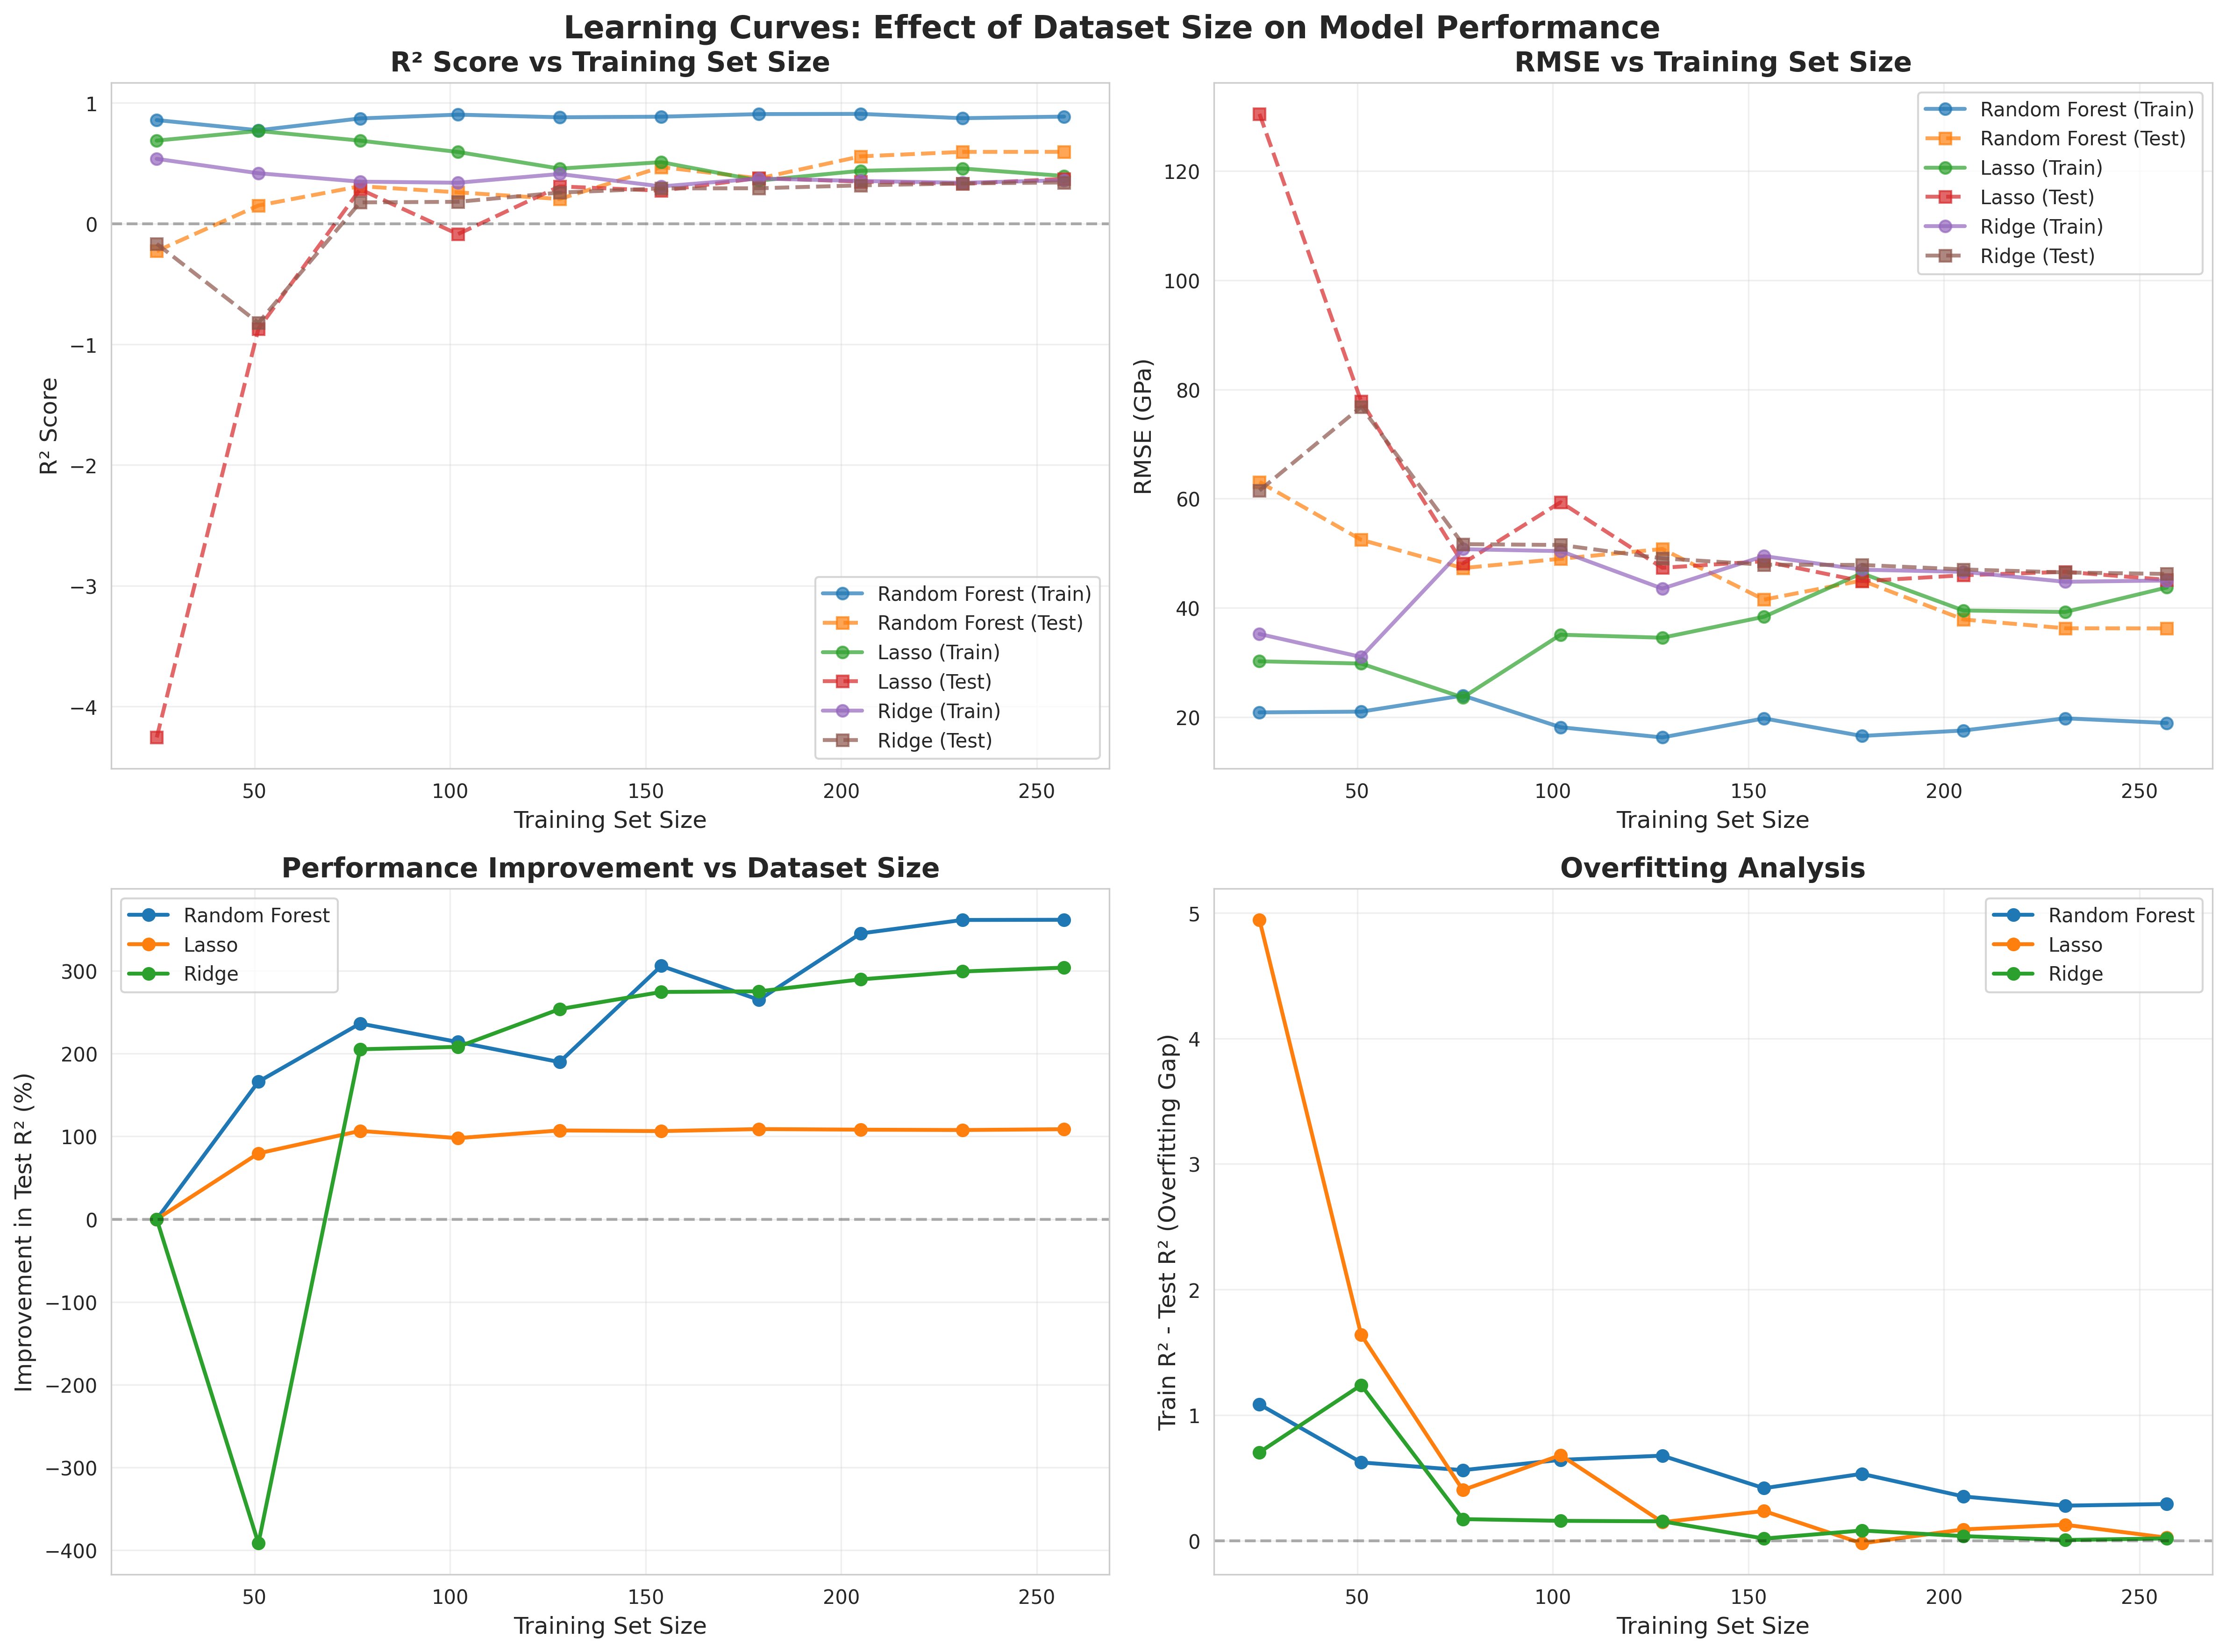
\includegraphics[width=0.85\textwidth]{figures/learning_curves.png}
\caption{Learning curves showing training and validation performance over epochs for selected models. The curves demonstrate convergence behavior and help identify optimal stopping points to prevent overfitting.}
\label{fig:learning_curves}
\end{figure}

\section{Results and Discussion}

On the initial 322-sample dataset, random forest provides the best baseline performance with test $R^2 \approx 0.57$ and RMSE of about 37.5~GPa. After hyperparameter optimization, SVR reaches $R^2 \approx 0.59$ with RMSE of about 36.2~GPa. When focusing on an experimental-only subset (roughly 109 samples), an optimized gradient boosting model achieves $R^2 \approx 0.67$, indicating good predictive power given the heterogeneity and limited size of the dataset. Among the advanced architectures, the composition-based Transformer (HEATransformer) achieves the best performance with test $R^2 \approx 0.62$ with RMSE of about 34.9~GPa and MAE of about 26.2~GPa on the same dataset, demonstrating superior performance and suggesting that sequence-based attention mechanisms can effectively capture compositional relationships in HEA/MPEA systems.

\begin{table}[htbp]
\centering
\caption{Model performance comparison on the 322-sample experimental dataset. Performance metrics include coefficient of determination ($R^2$), root mean squared error (RMSE), and mean absolute error (MAE).}
\label{tab:model_performance}
\begin{tabular}{lccc}
\hline
Model & Test $R^2$ & Test RMSE (GPa) & Test MAE (GPa) \\
\hline
Random Forest & 0.57 & 37.5 & 25.9 \\
SVR (optimized) & 0.59 & 36.2 & -- \\
Gradient Boosting (exp.\ only) & 0.67 & 49.7 & 37.1 \\
MLFFNN & 0.49 & 40.5 & 29.0 \\
Lasso & 0.37 & 45.1 & 31.3 \\
Linear & 0.36 & 45.5 & 32.6 \\
SVR (baseline) & 0.36 & 45.6 & 29.1 \\
Ridge & 0.34 & 46.2 & 32.0 \\
KNN & 0.02 & 56.3 & 44.4 \\
Polynomial & $<0$ & 97.5 & 61.1 \\
Transformer (HEATransformer) & 0.62 & 34.9 & 26.2 \\
\hline
\end{tabular}
\end{table}

\begin{figure}[htbp]
\centering
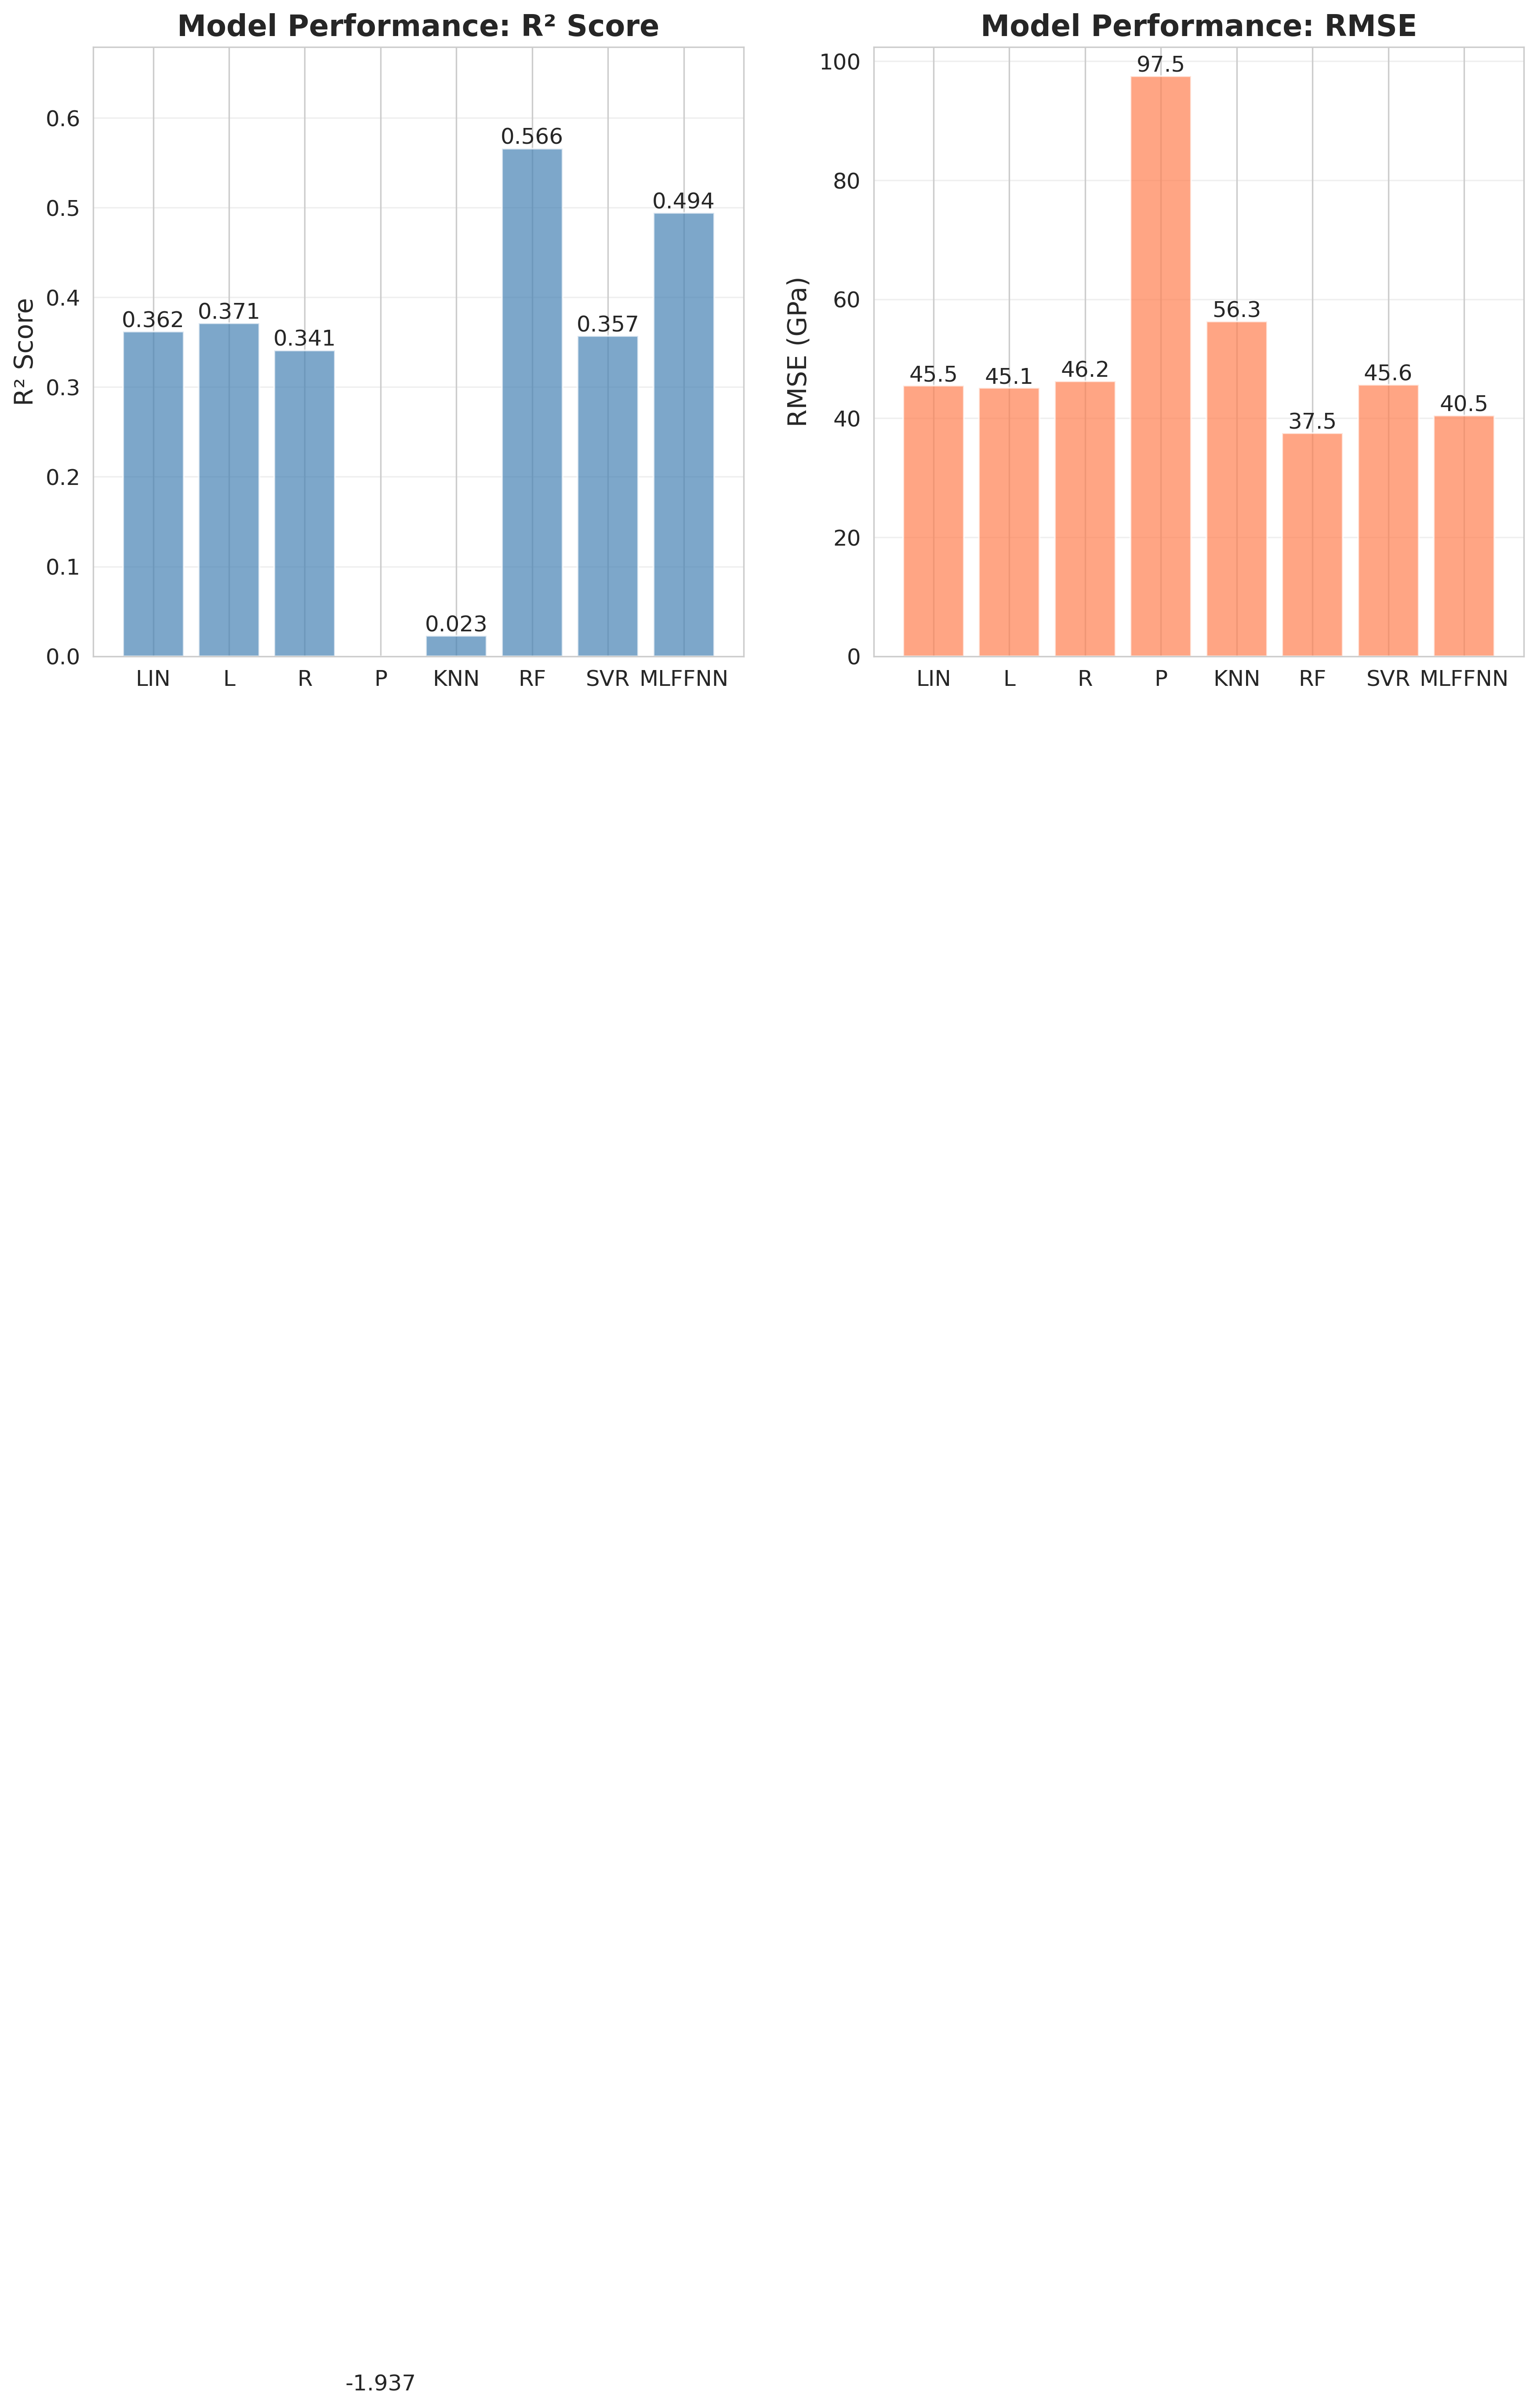
\includegraphics[width=0.85\textwidth]{figures/model_performance_comparison.png}
\caption{Comparison of model performance metrics (R$^2$ and RMSE) across different machine-learning algorithms. The optimized SVR and Gradient Boosting models show the best performance, with R$^2$ values of approximately 0.59 and 0.67, respectively.}
\label{fig:model_performance}
\end{figure}

\begin{figure}[htbp]
\centering
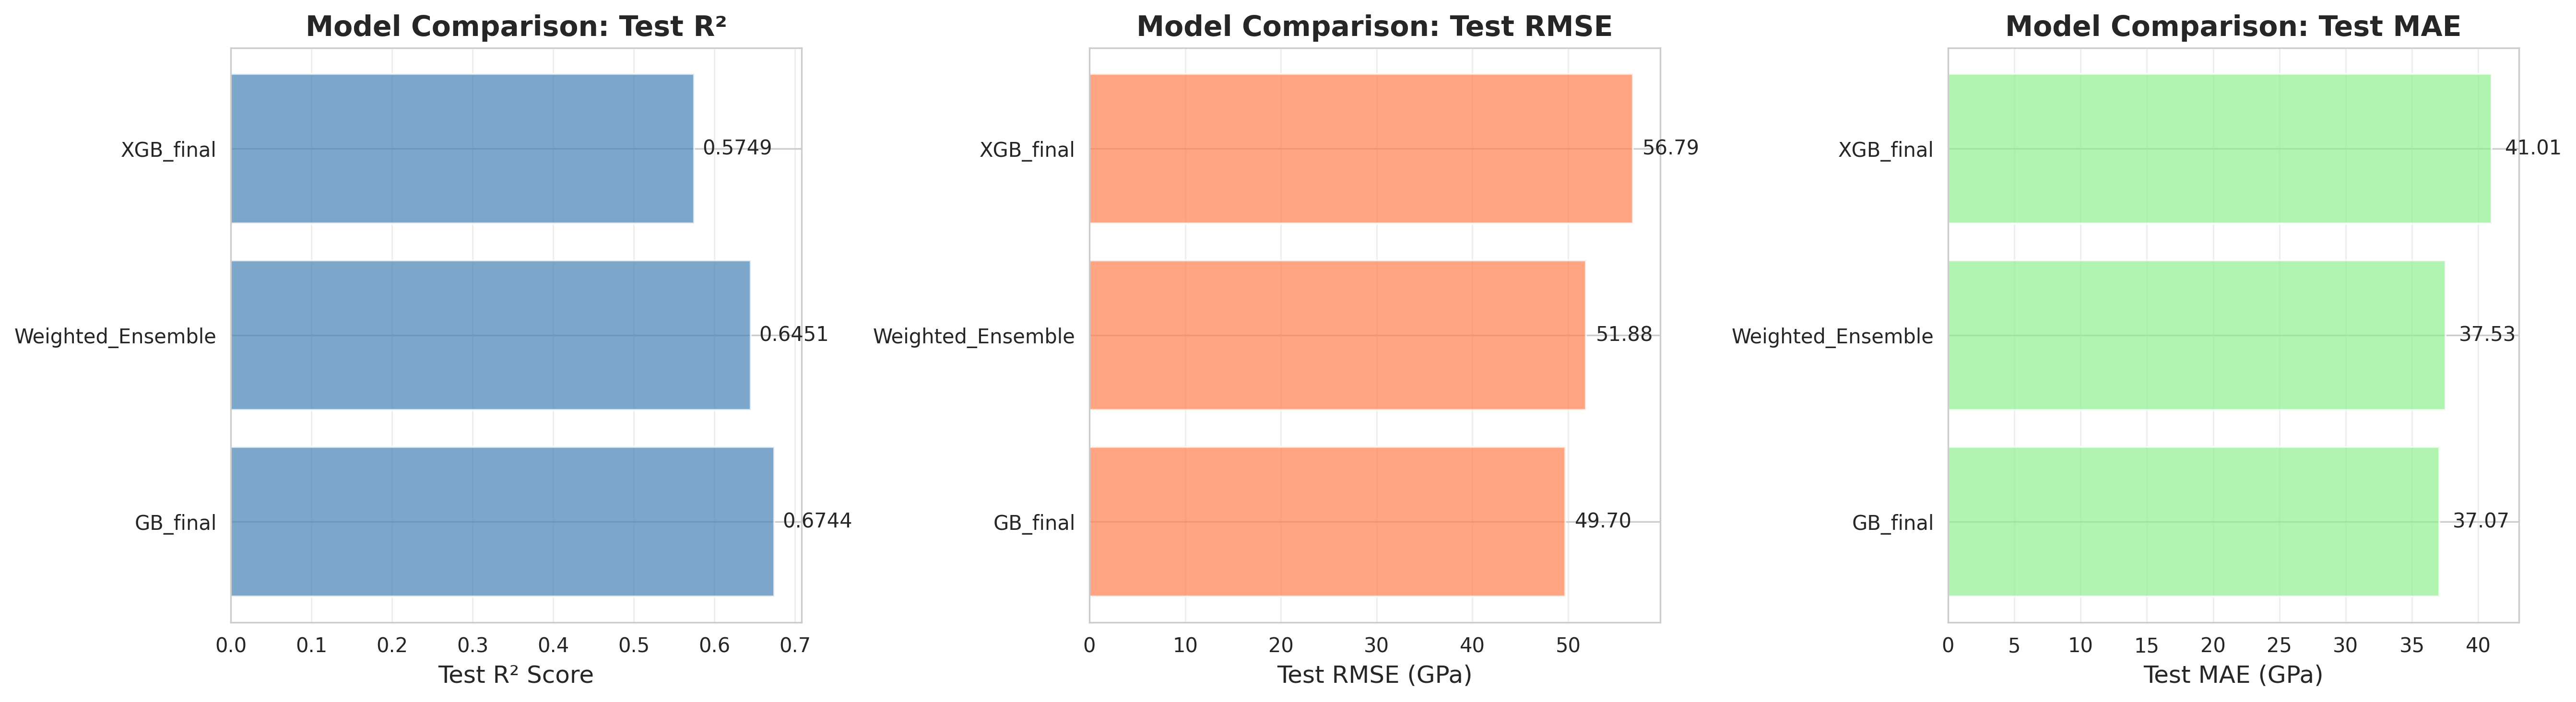
\includegraphics[width=0.85\textwidth]{figures/model_comparison_all.png}
\caption{Comprehensive comparison of all models showing performance across different metrics and data subsets. This visualization helps identify the best-performing models for different use cases.}
\label{fig:model_comparison_all}
\end{figure}

\begin{figure}[htbp]
\centering
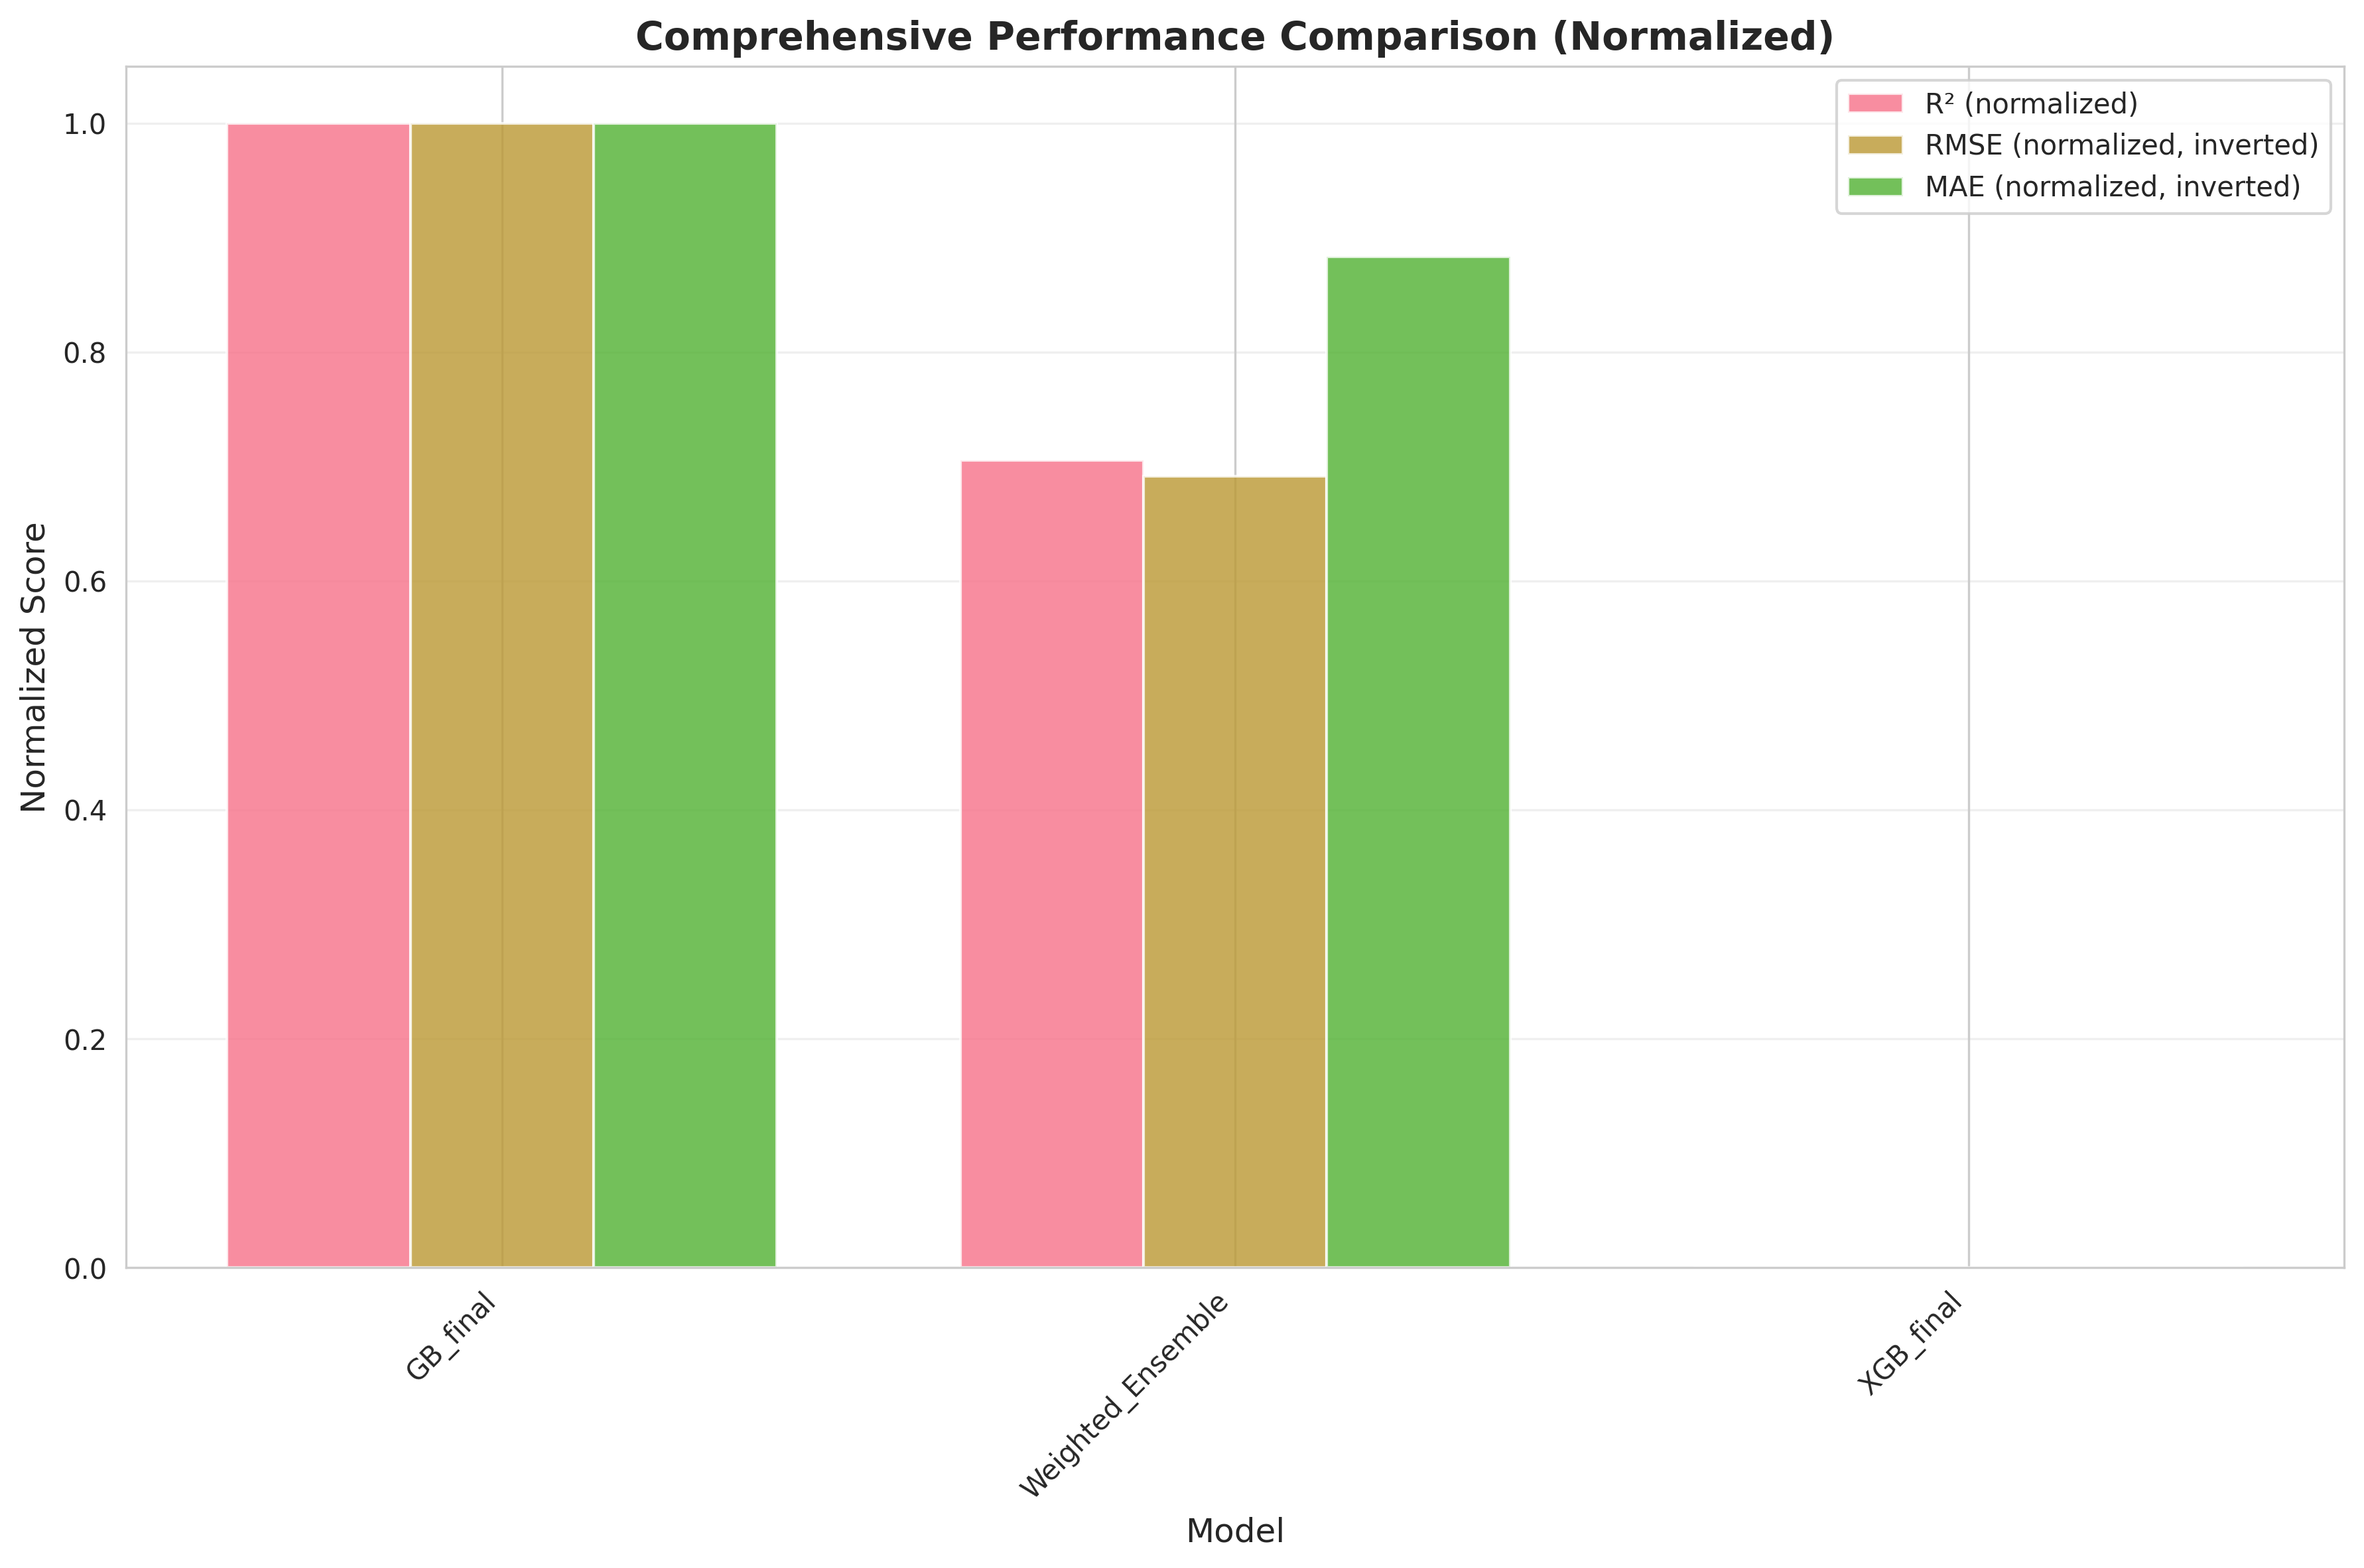
\includegraphics[width=0.85\textwidth]{figures/performance_metrics_comparison.png}
\caption{Detailed comparison of performance metrics (R$^2$, RMSE, MAE) for all evaluated models, highlighting the trade-offs between different evaluation criteria.}
\label{fig:performance_metrics}
\end{figure}

Feature-importance analyses from random forest and gradient boosting consistently identify the Ti composition fraction, average electronegativity, VEC, Co composition fraction, and density as dominant contributors. These trends support intuitive design guidelines for tuning elastic modulus, such as leveraging Ti-rich, lower-density compositions to reduce stiffness while carefully balancing refractory elements that increase modulus.

\begin{figure}[htbp]
\centering
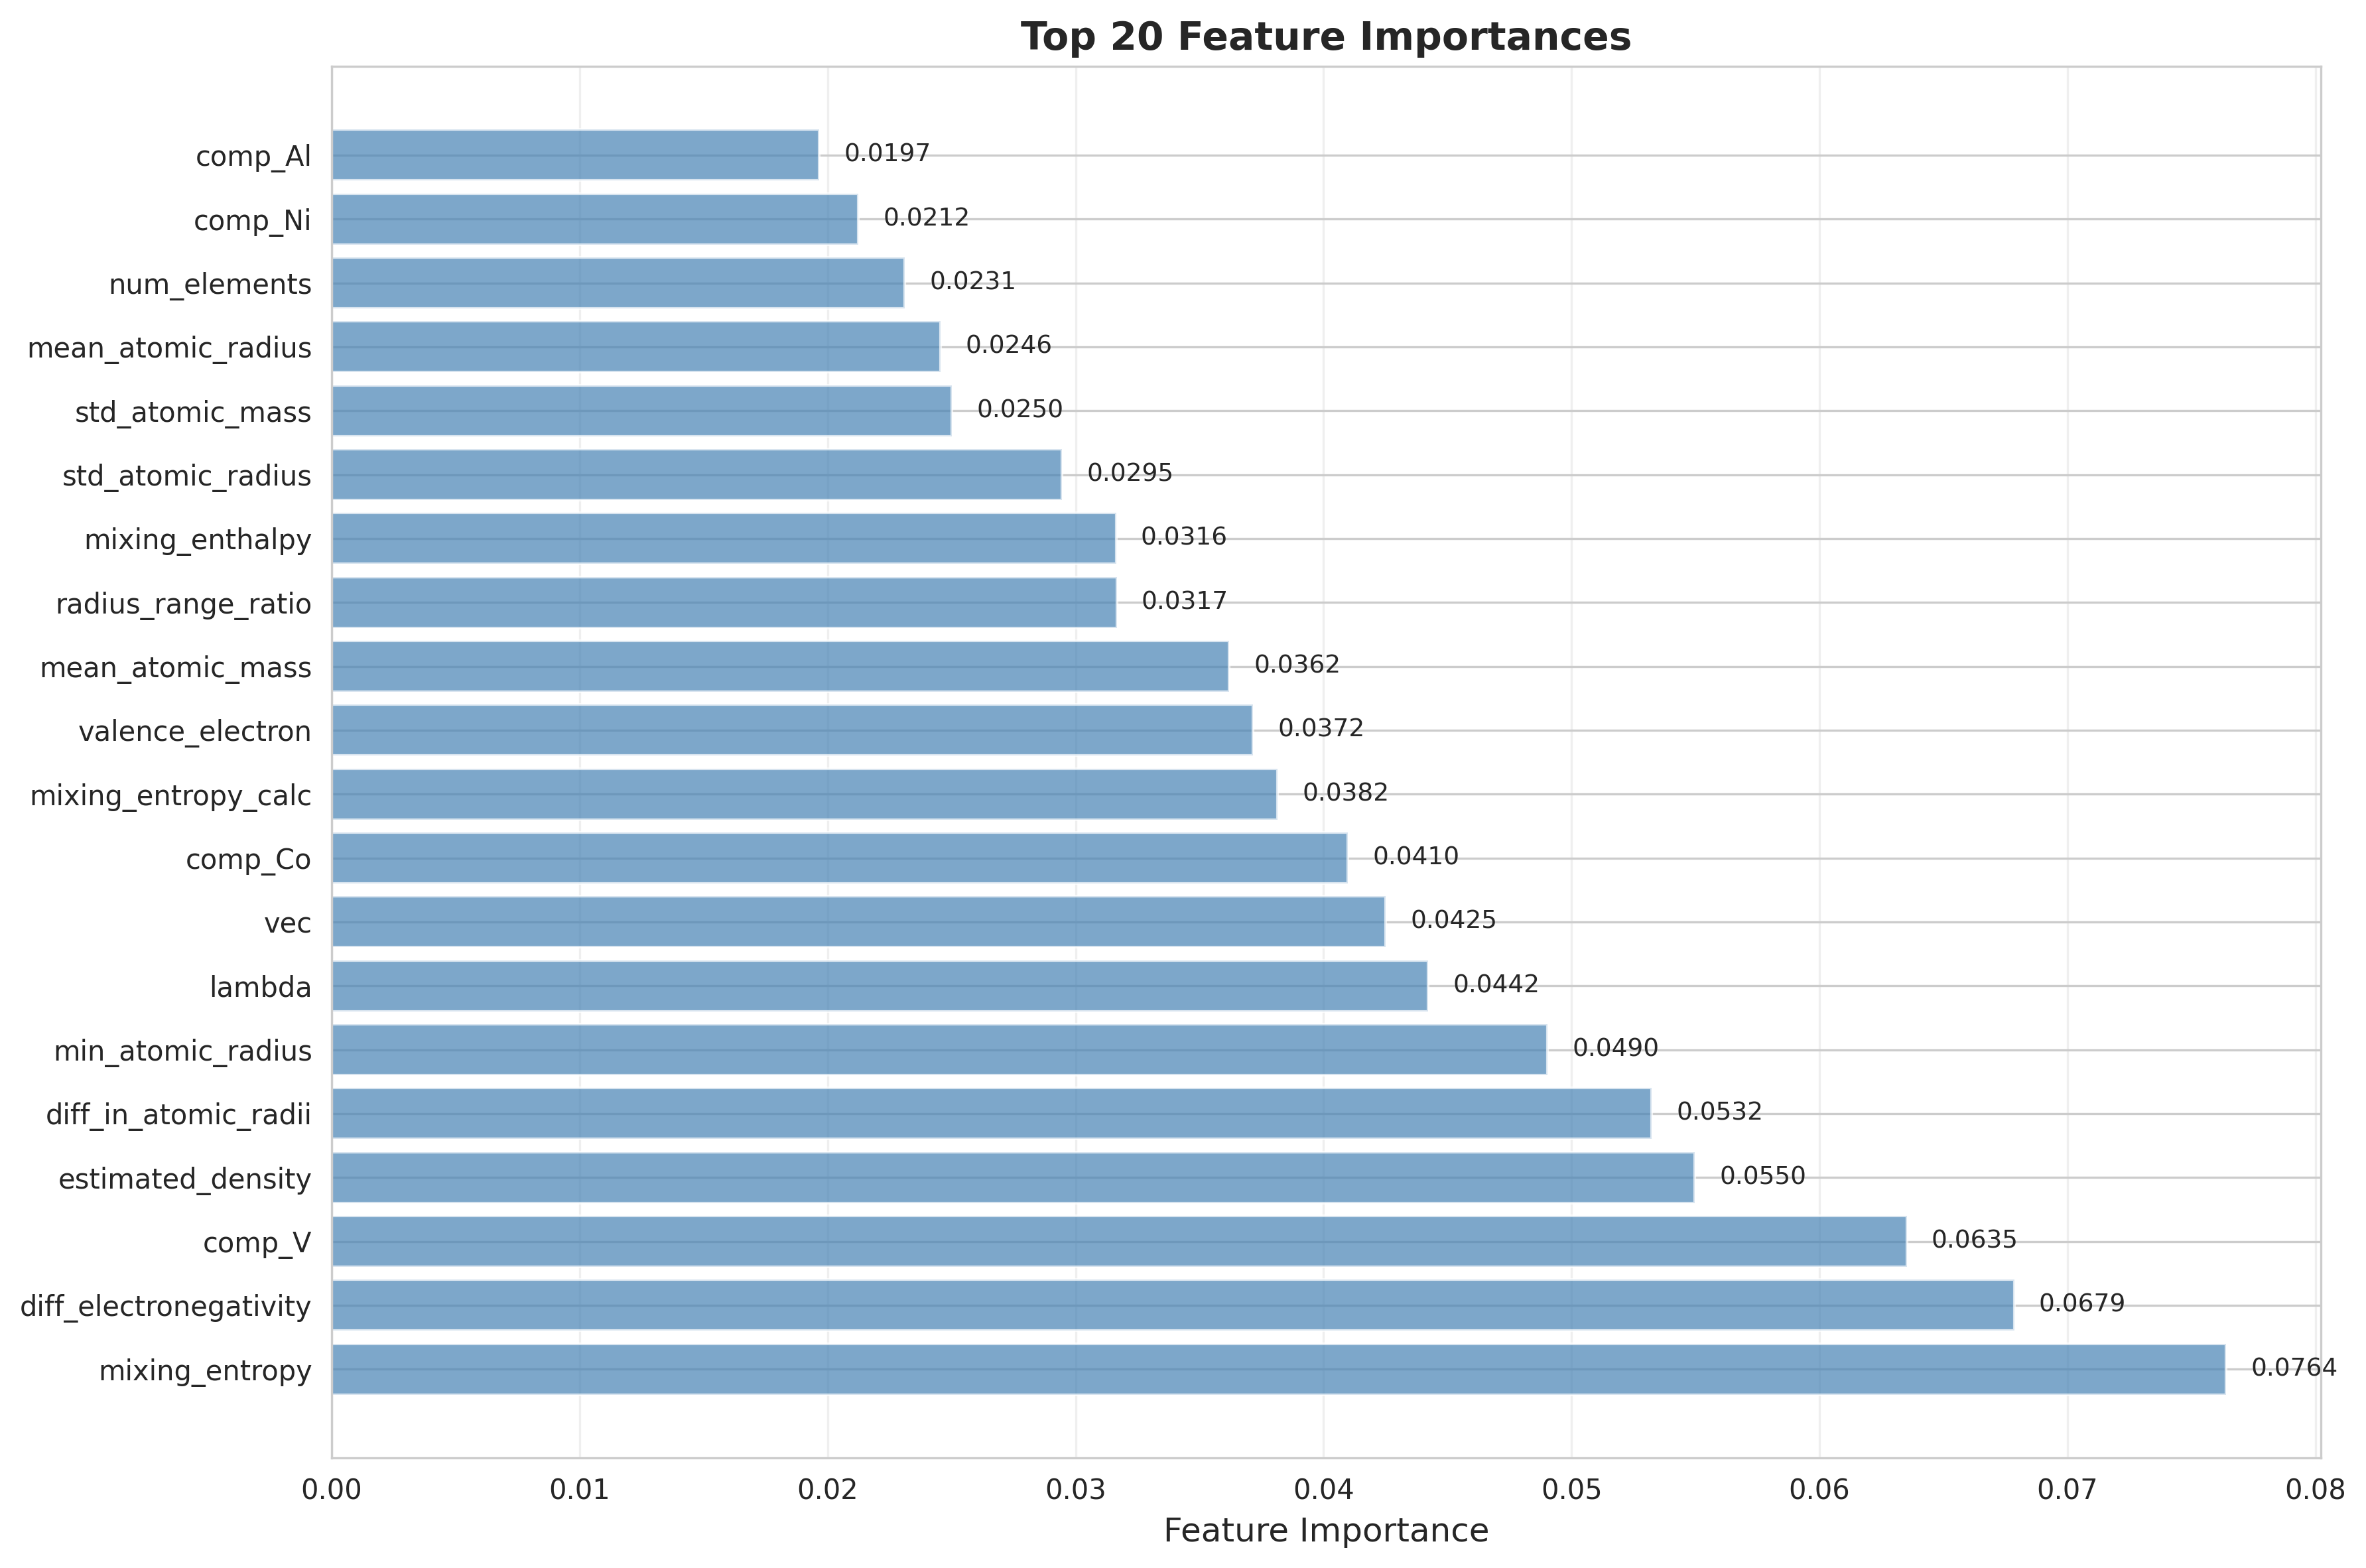
\includegraphics[width=0.85\textwidth]{figures/feature_importance.png}
\caption{Feature importance analysis from Random Forest regression. The Ti composition fraction (\texttt{comp\_Ti}) shows the highest importance (approximately 16--17\%), followed by average electronegativity, valence electron concentration (VEC), Co composition fraction, and density.}
\label{fig:feature_importance}
\end{figure}

\begin{figure}[htbp]
\centering
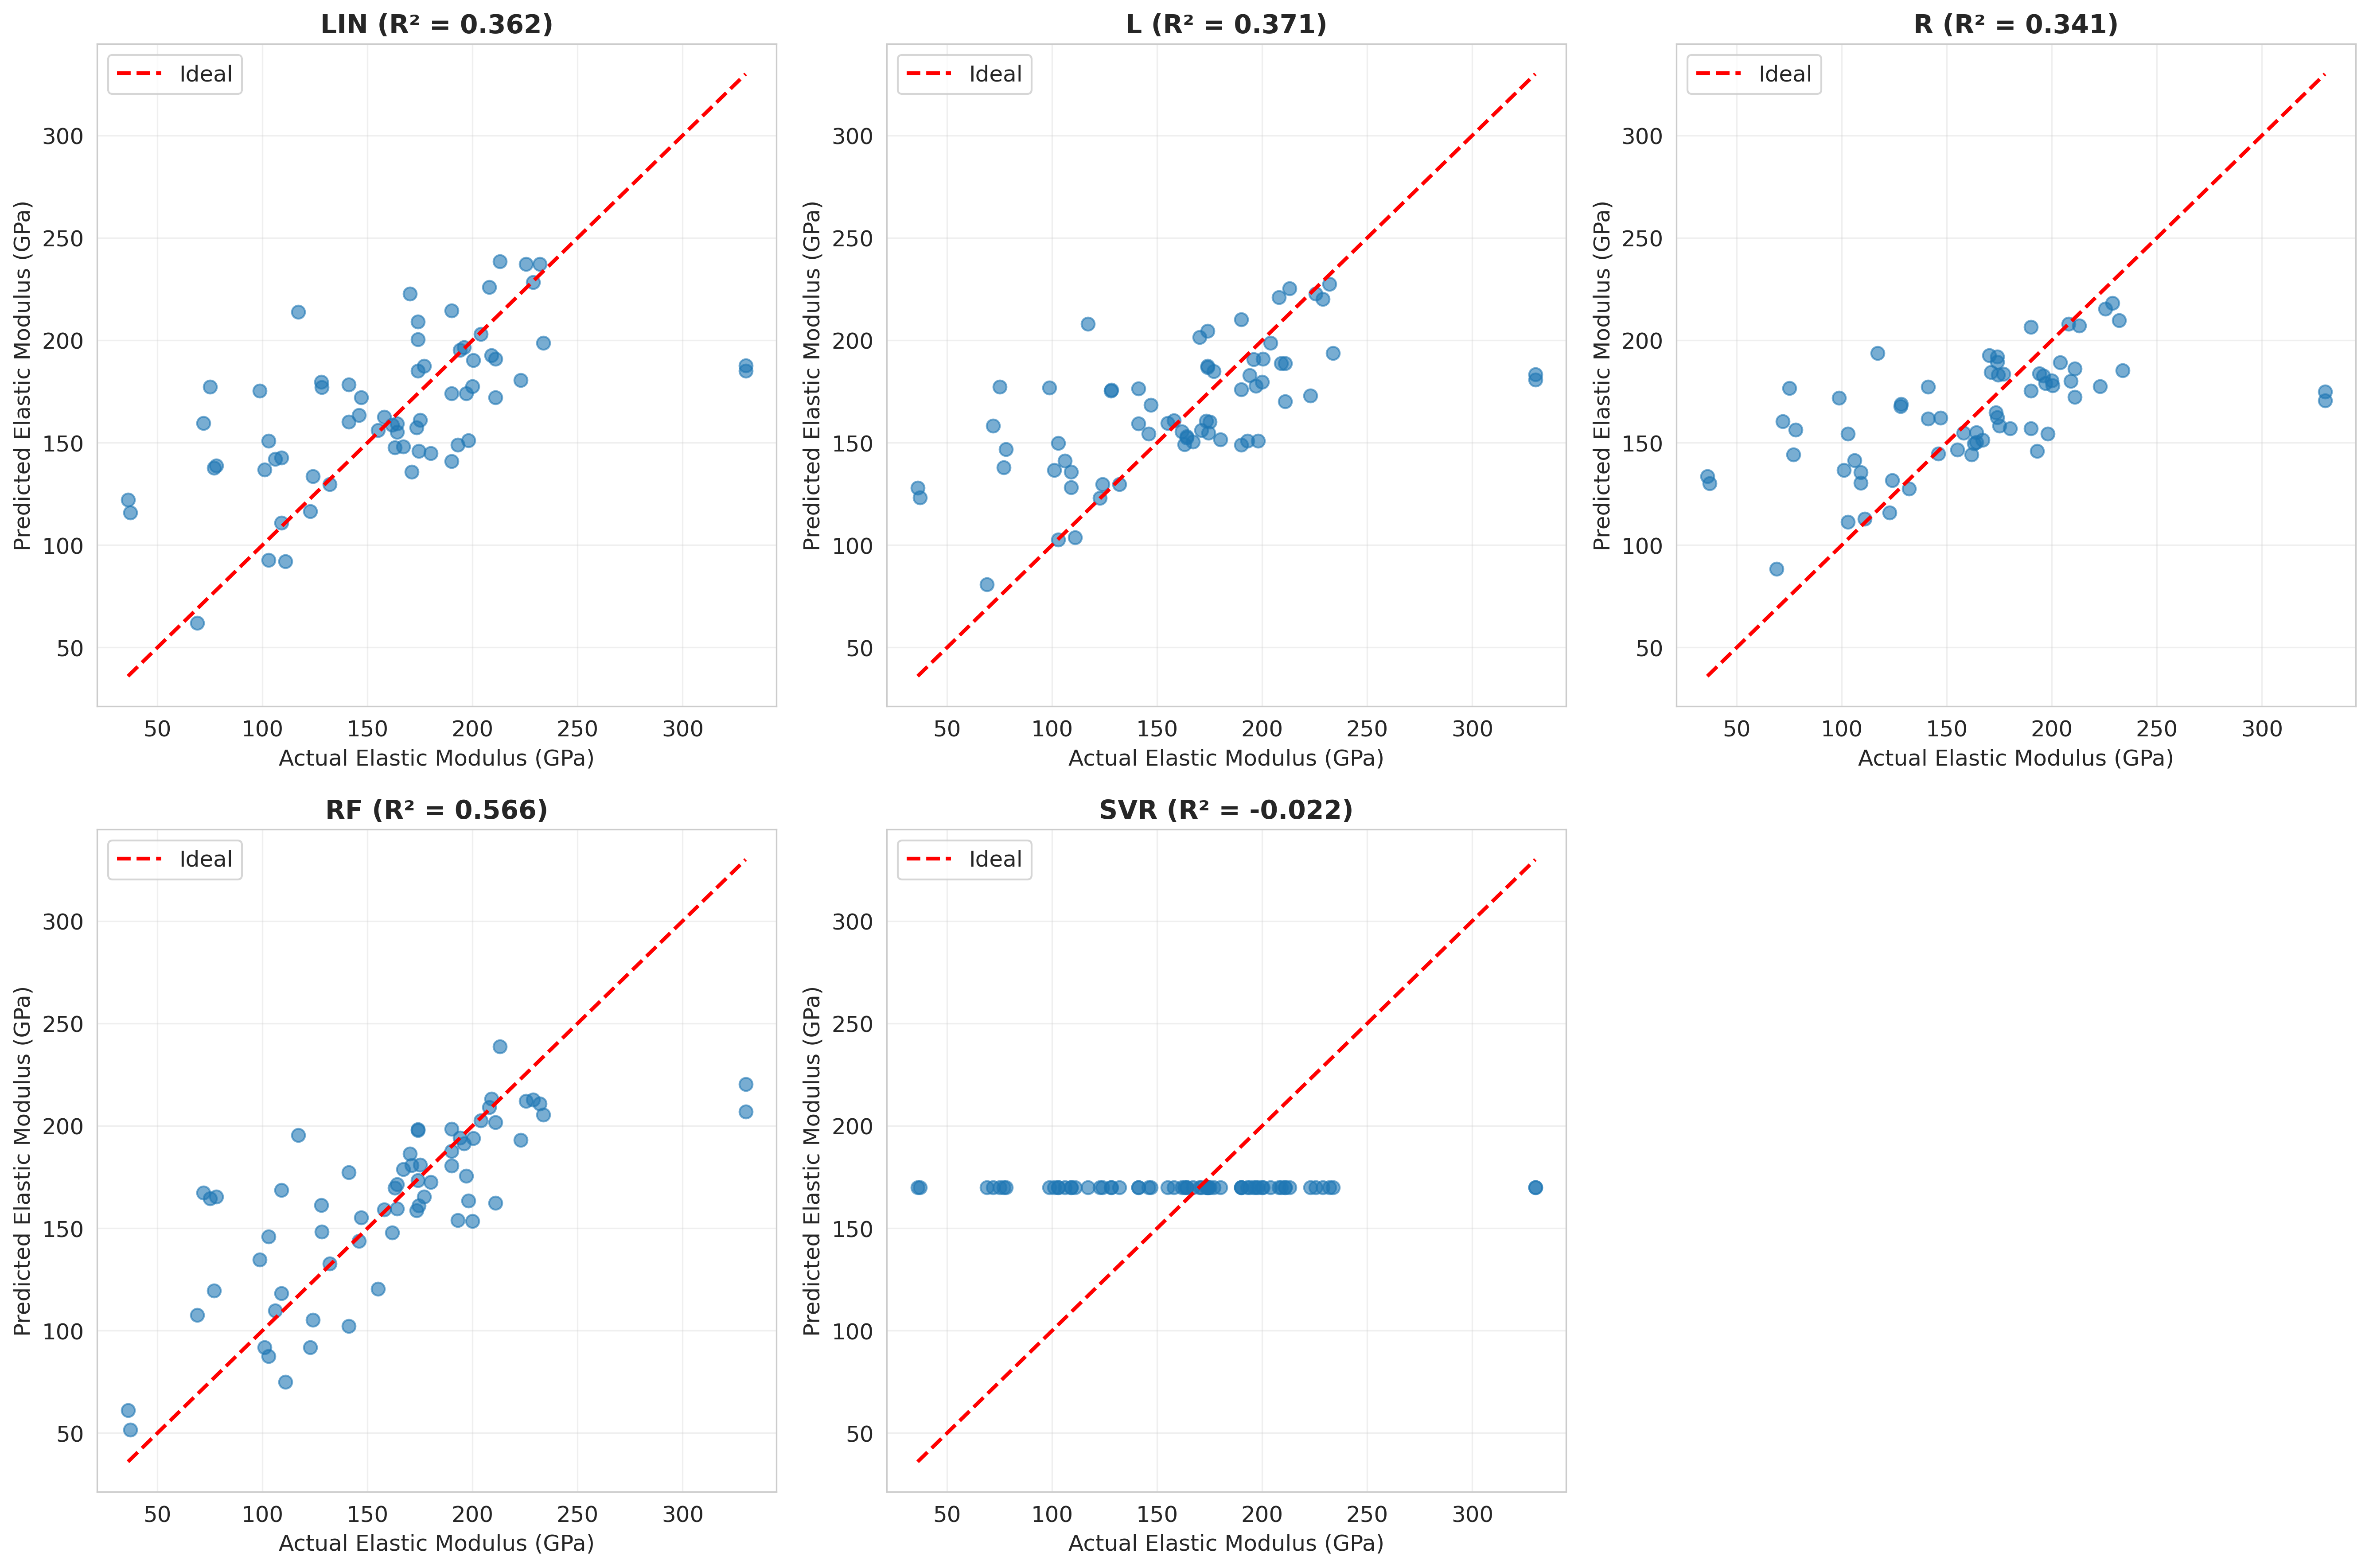
\includegraphics[width=0.85\textwidth]{figures/predicted_vs_actual.png}
\caption{Predicted vs.\ actual elastic modulus values for the optimized SVR model on the 322-sample dataset. The diagonal line represents perfect prediction. Most predictions cluster around the diagonal, indicating reasonable model calibration, though some scatter is present, particularly at the extremes of the modulus range.}
\label{fig:predicted_vs_actual}
\end{figure}

\begin{figure}[htbp]
\centering
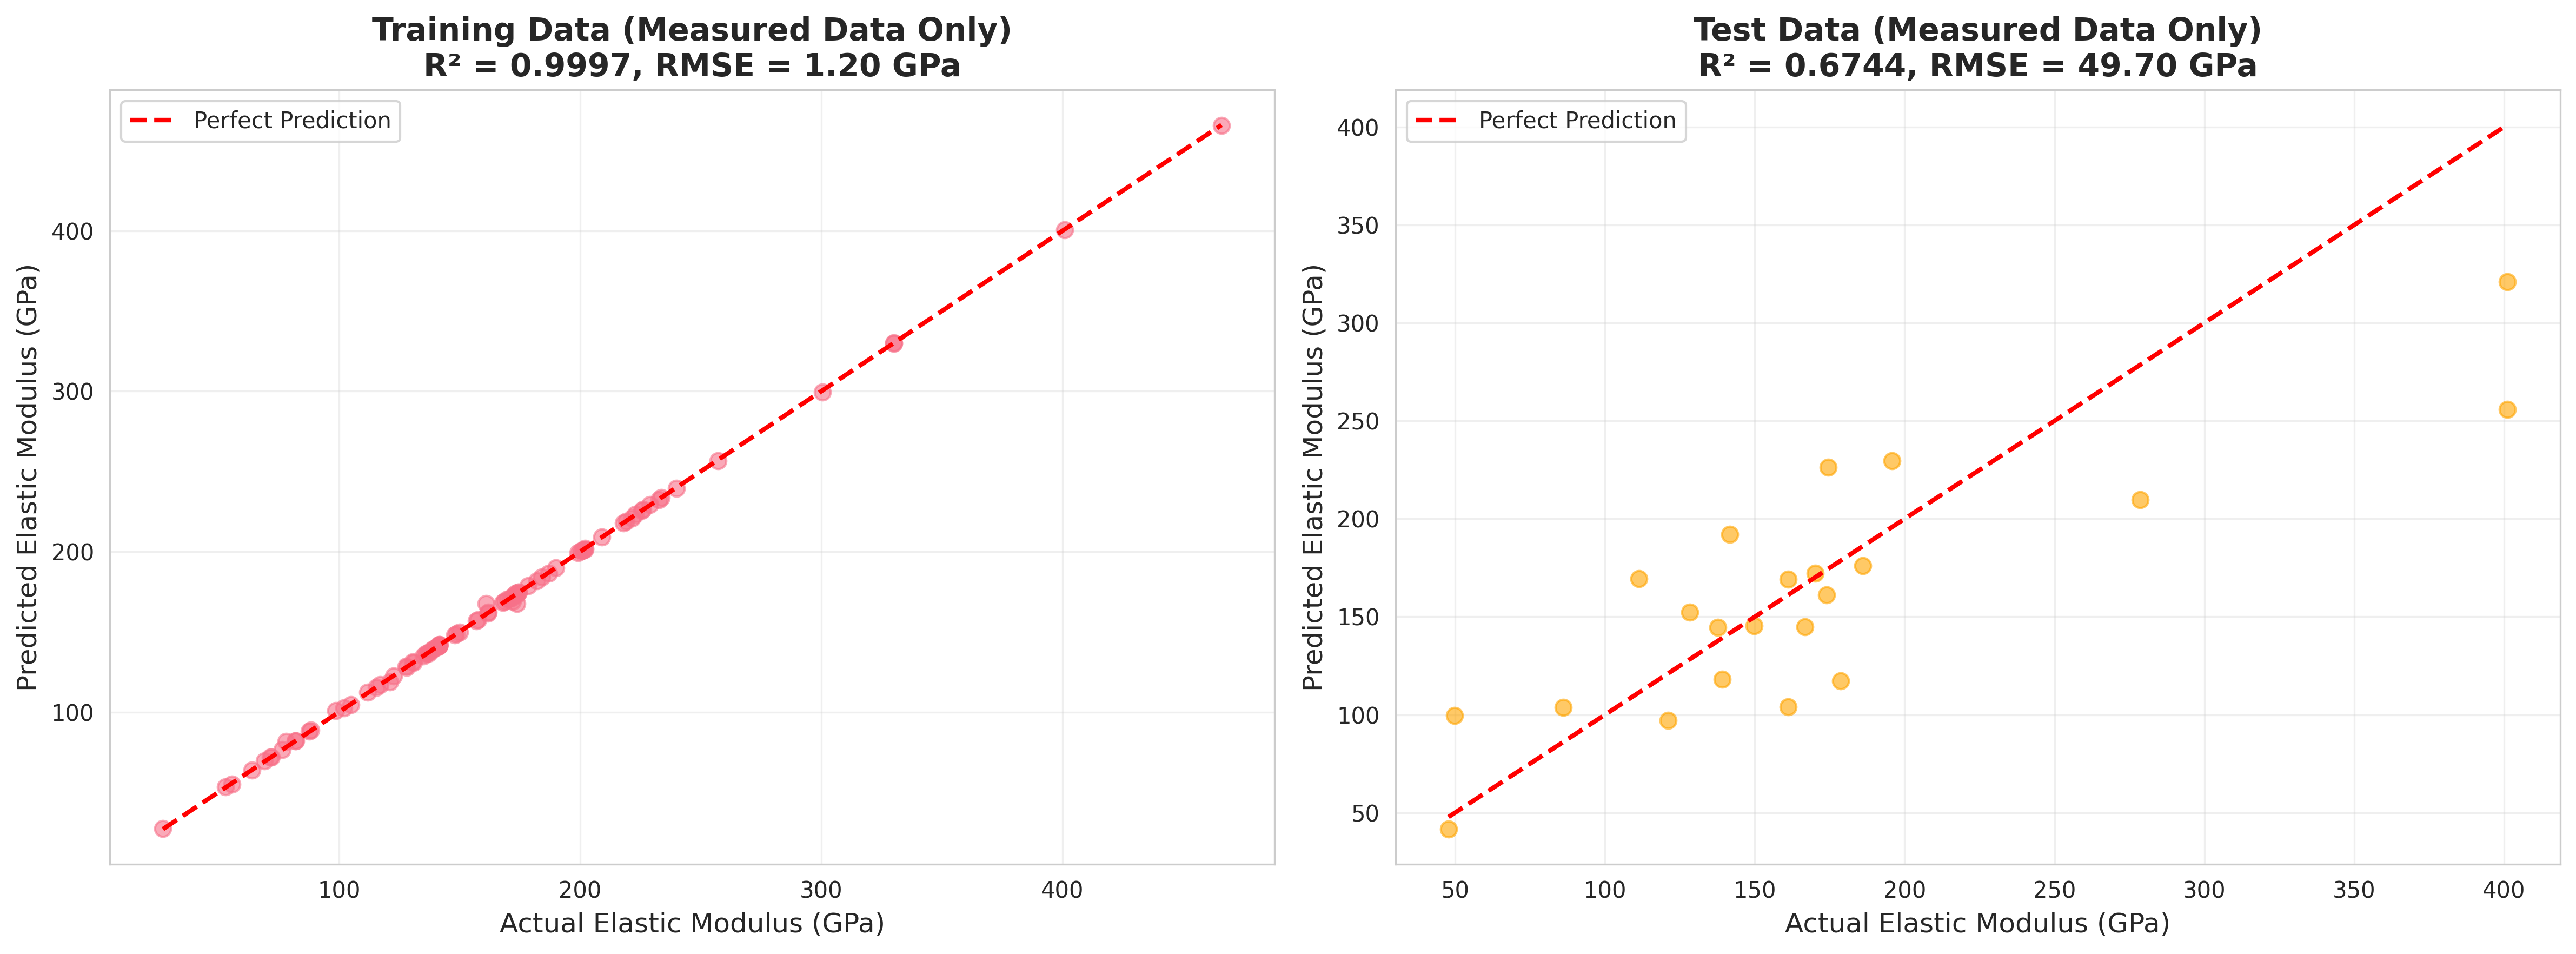
\includegraphics[width=0.85\textwidth]{figures/predicted_vs_actual_(measured_data_only).png}
\caption{Predicted vs.\ actual elastic modulus for models evaluated on the experimental-only subset. This comparison helps assess model performance when applied to purely experimental data, avoiding potential biases from computed values.}
\label{fig:predicted_vs_actual_measured}
\end{figure}

\begin{figure}[htbp]
\centering
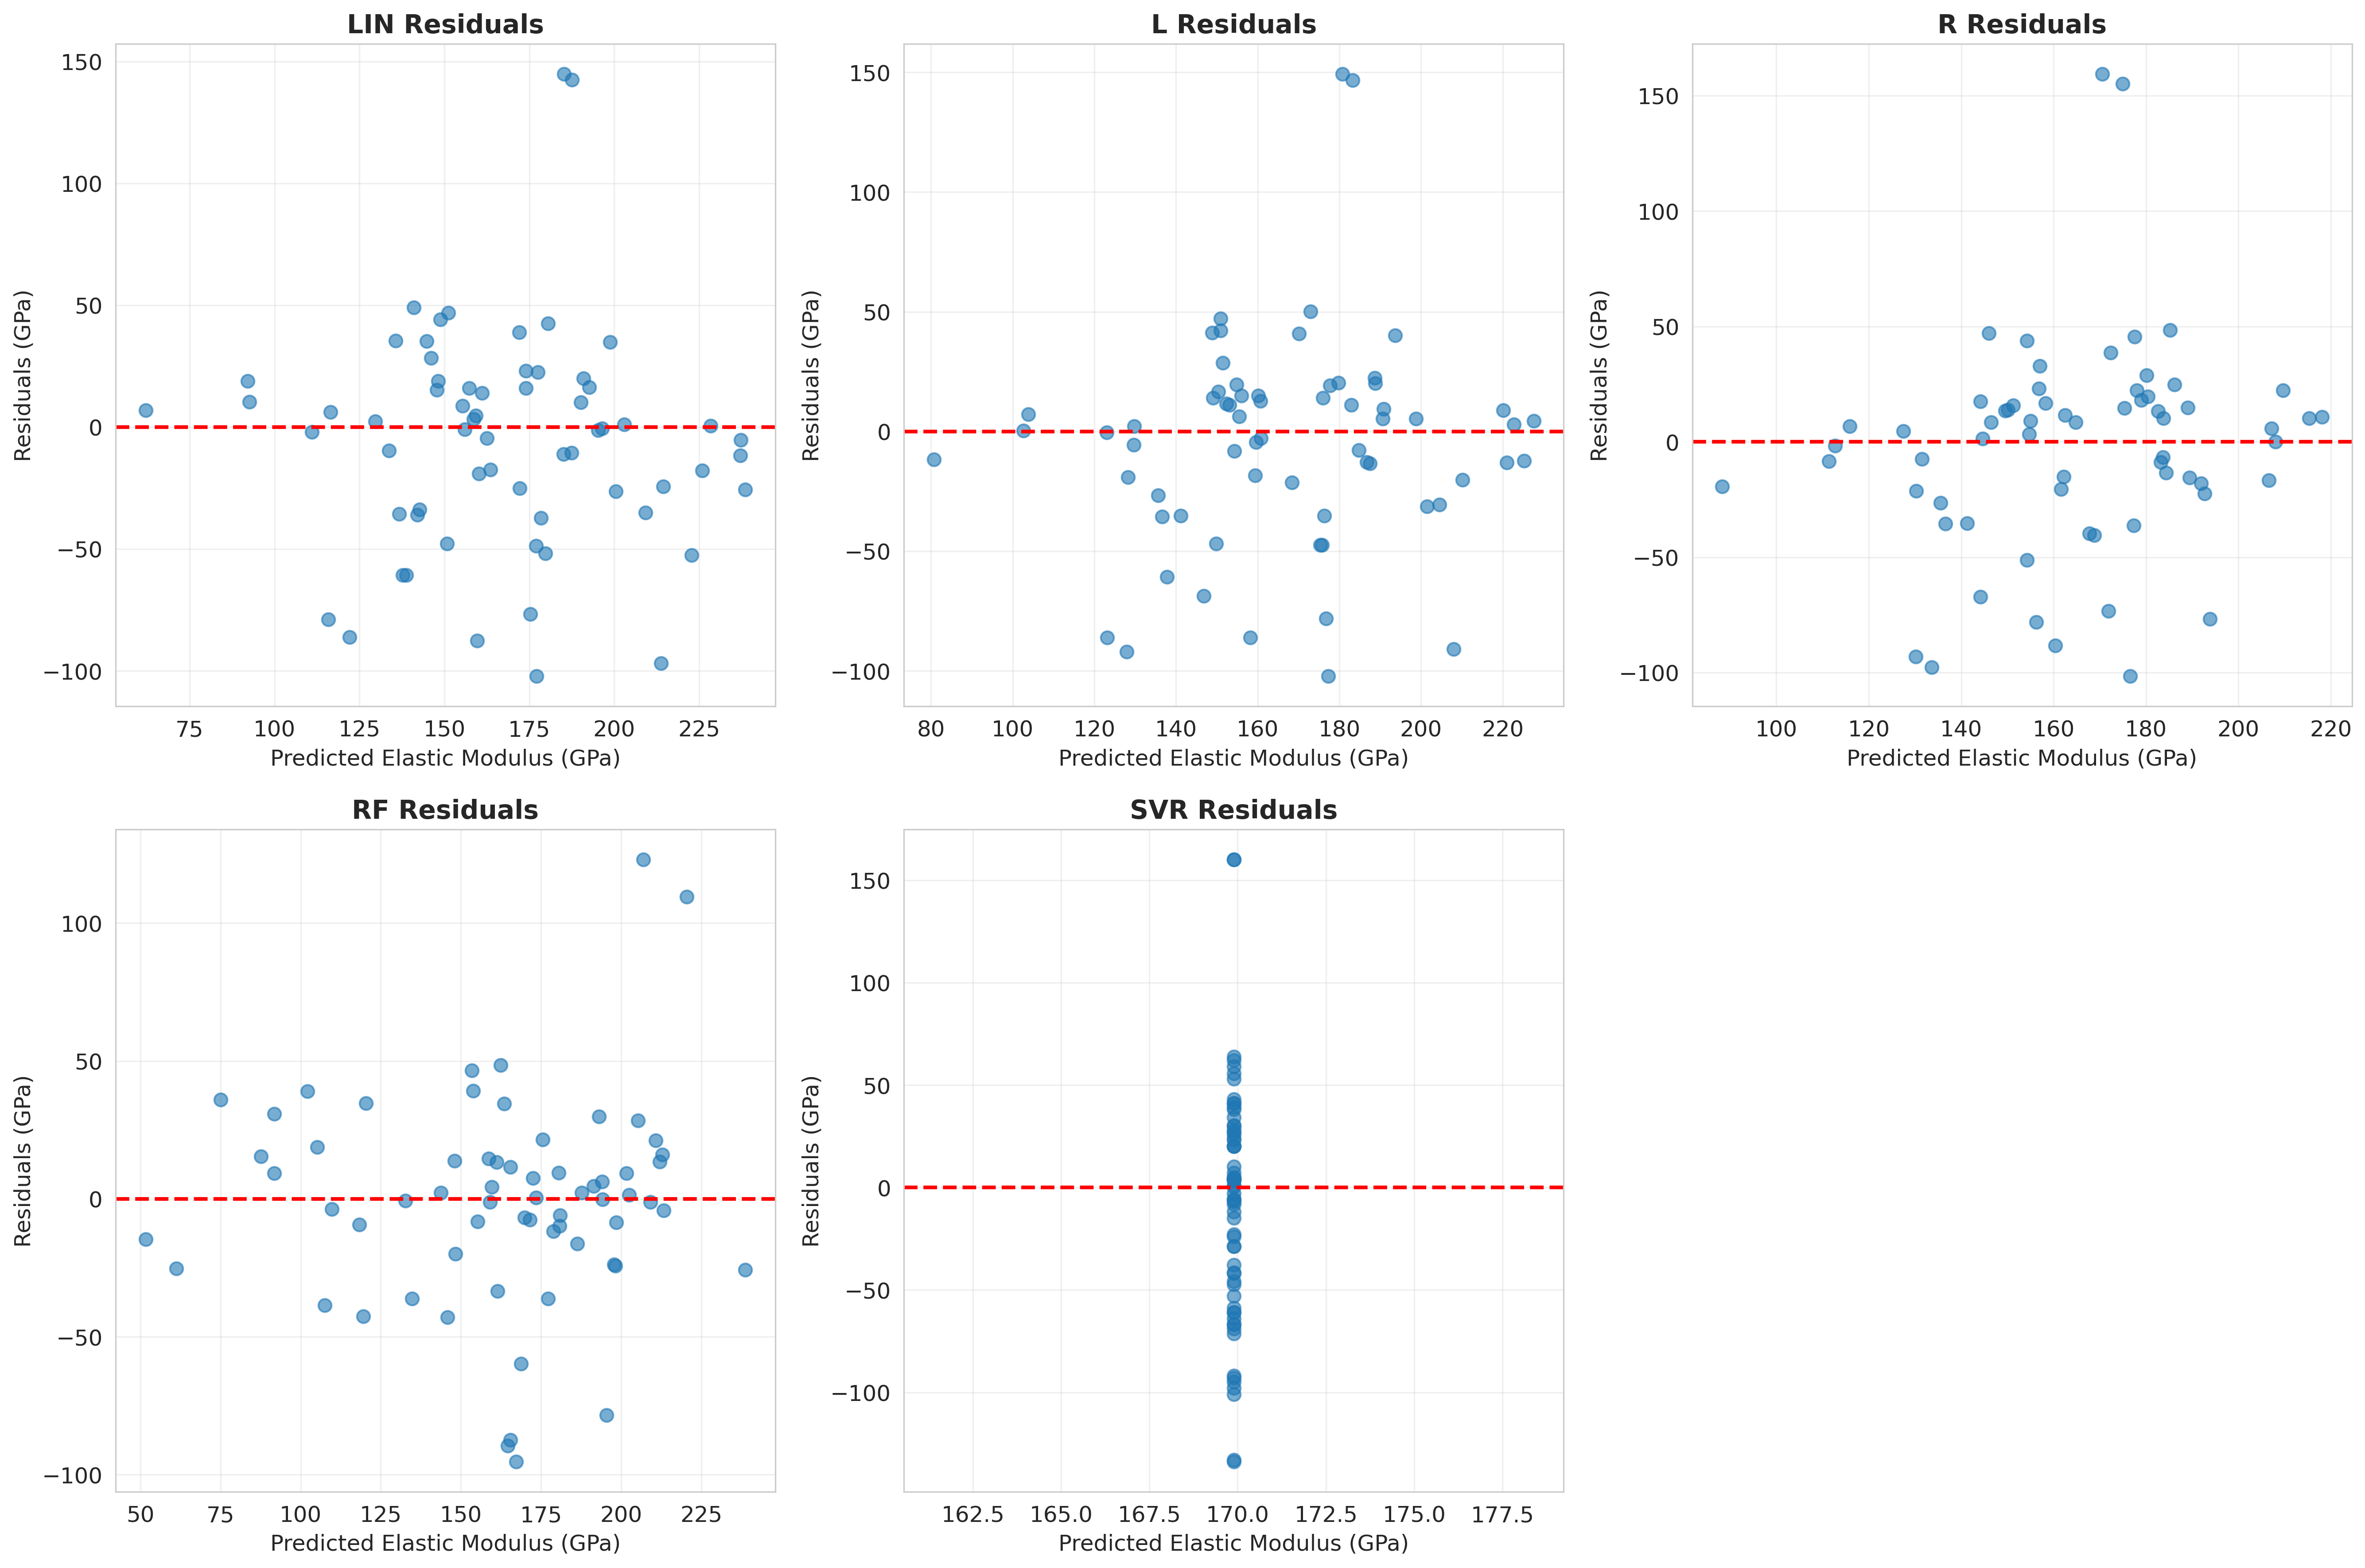
\includegraphics[width=0.85\textwidth]{figures/residuals_analysis.png}
\caption{Residual analysis for the optimized SVR model. The residuals are approximately centered around zero with no strong systematic trends, suggesting that the model captures the main relationships without severe bias. Larger errors tend to occur at the extremes of the modulus distribution.}
\label{fig:residuals}
\end{figure}

\begin{figure}[htbp]
\centering
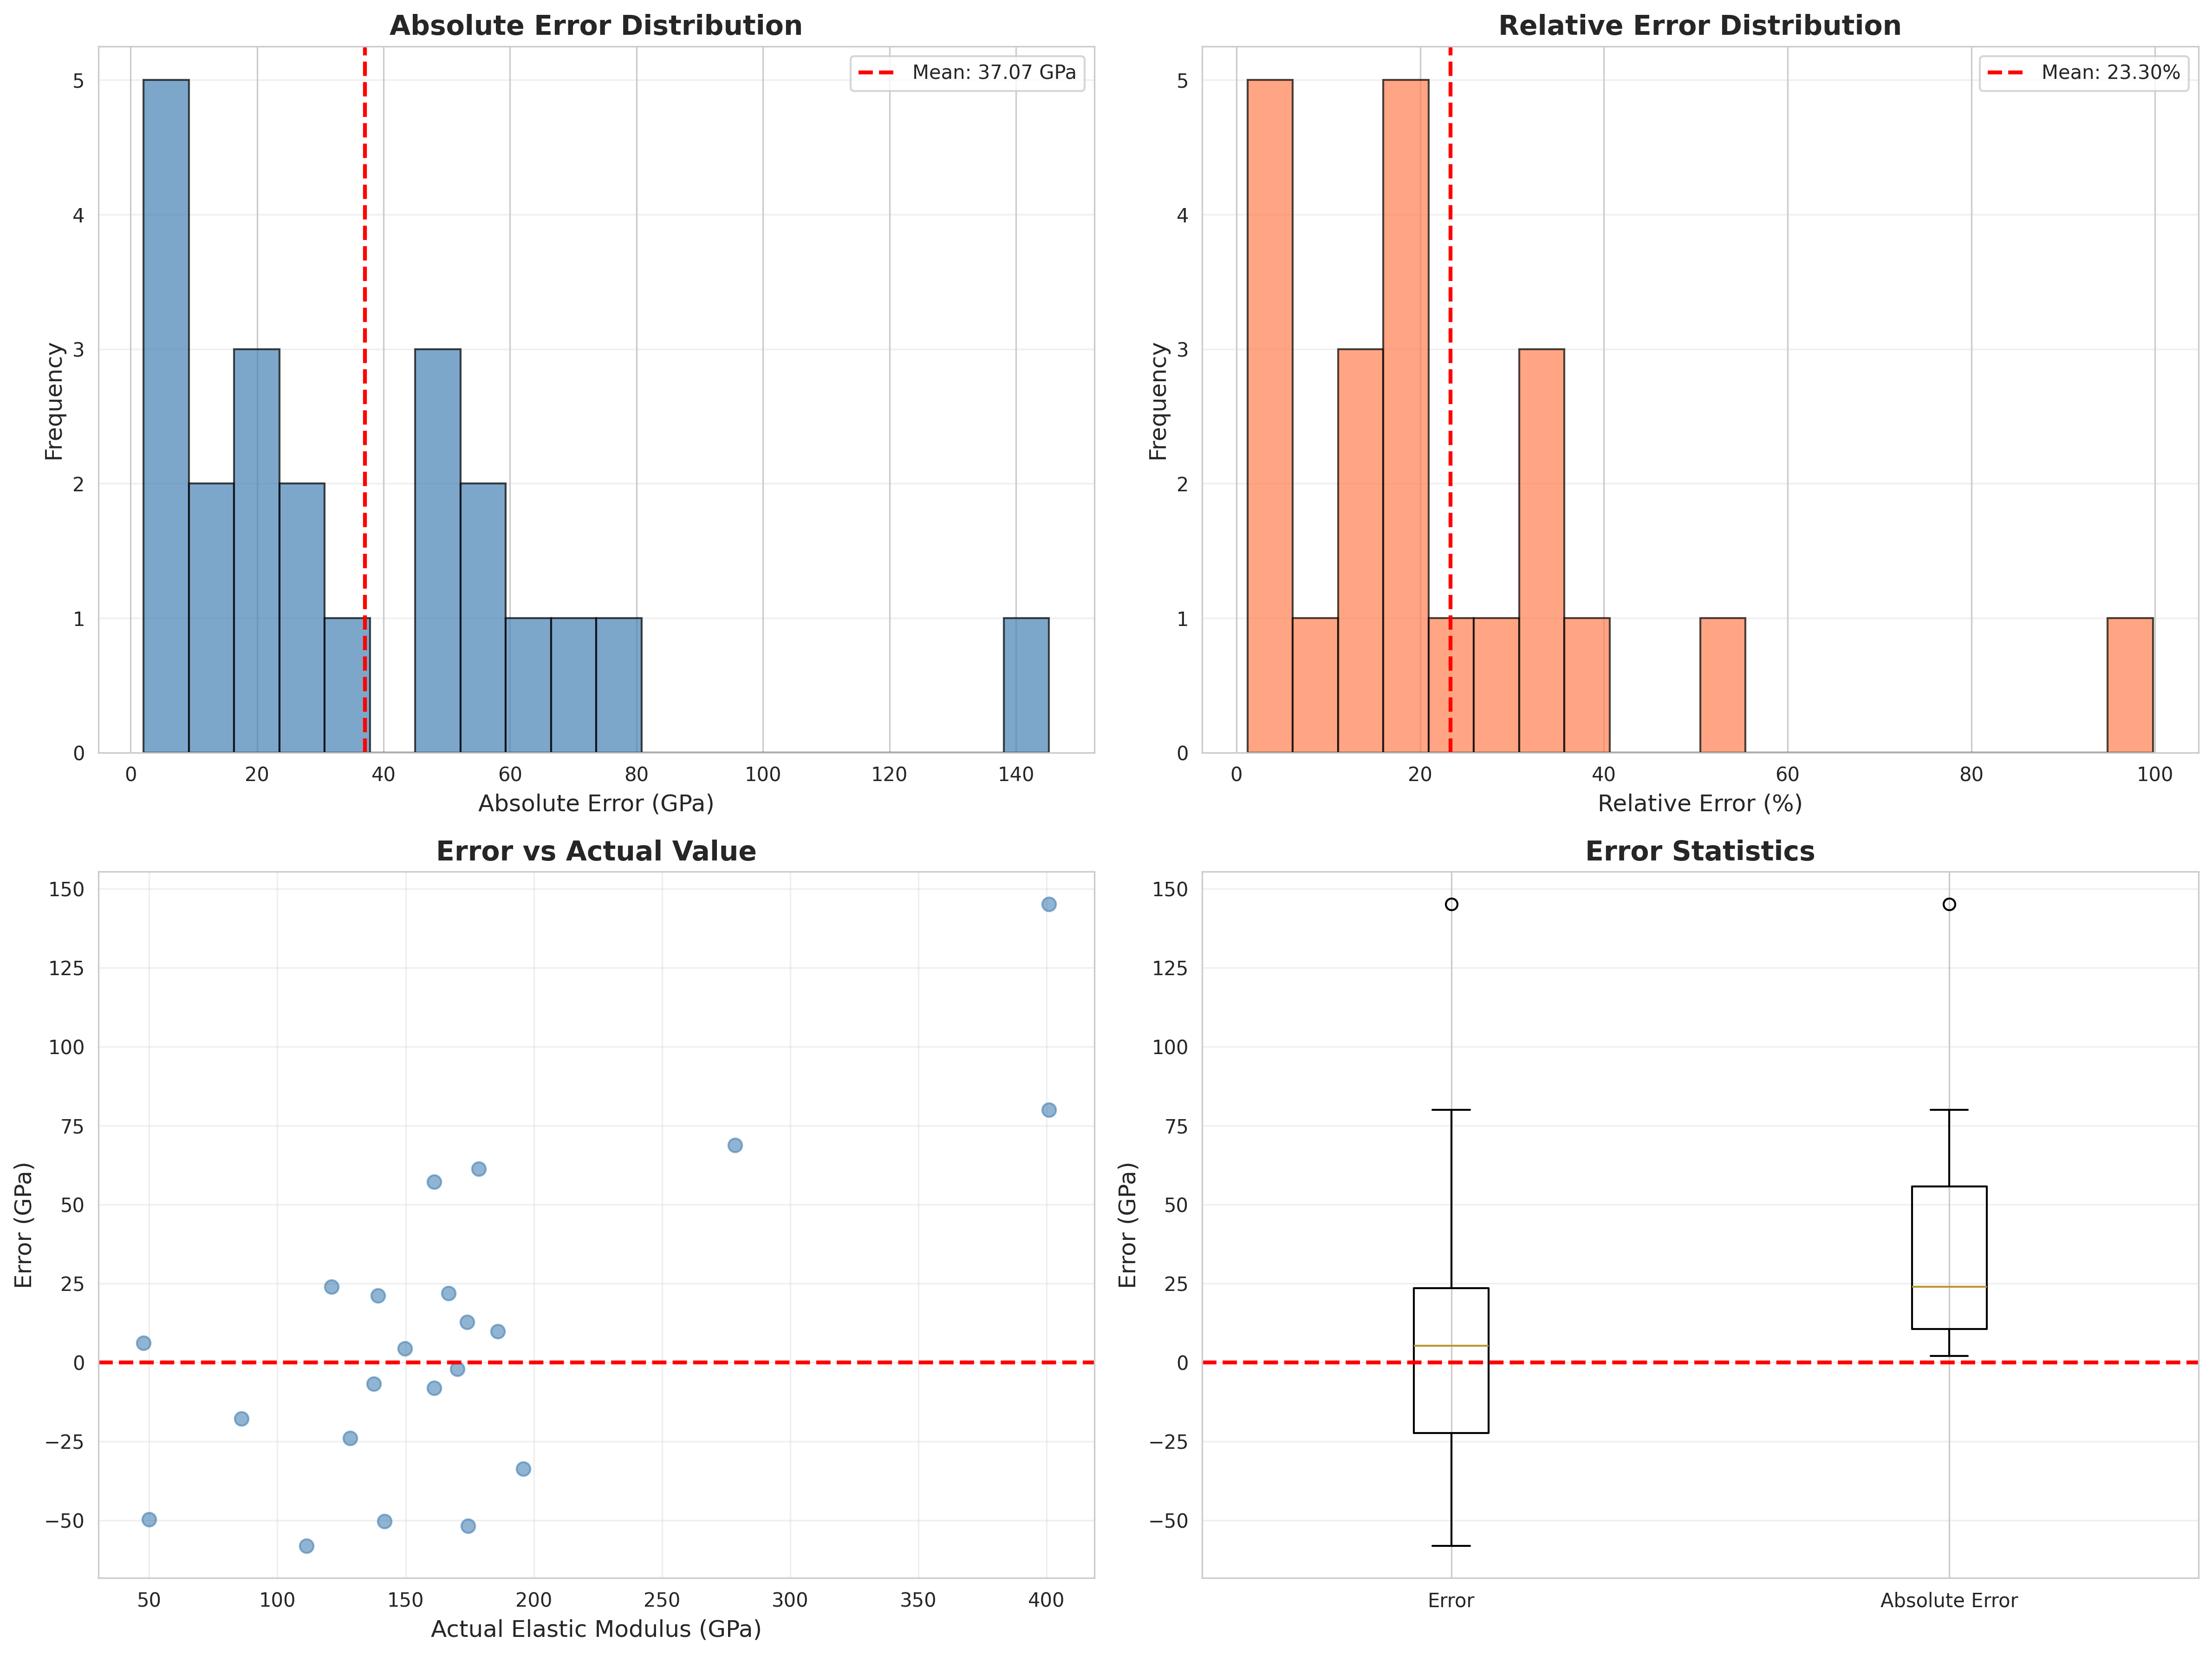
\includegraphics[width=0.85\textwidth]{figures/error_distribution.png}
\caption{Distribution of prediction errors across all models. The error distributions help identify systematic biases and assess the reliability of predictions for different modulus ranges.}
\label{fig:error_distribution}
\end{figure}

\begin{figure}[htbp]
\centering
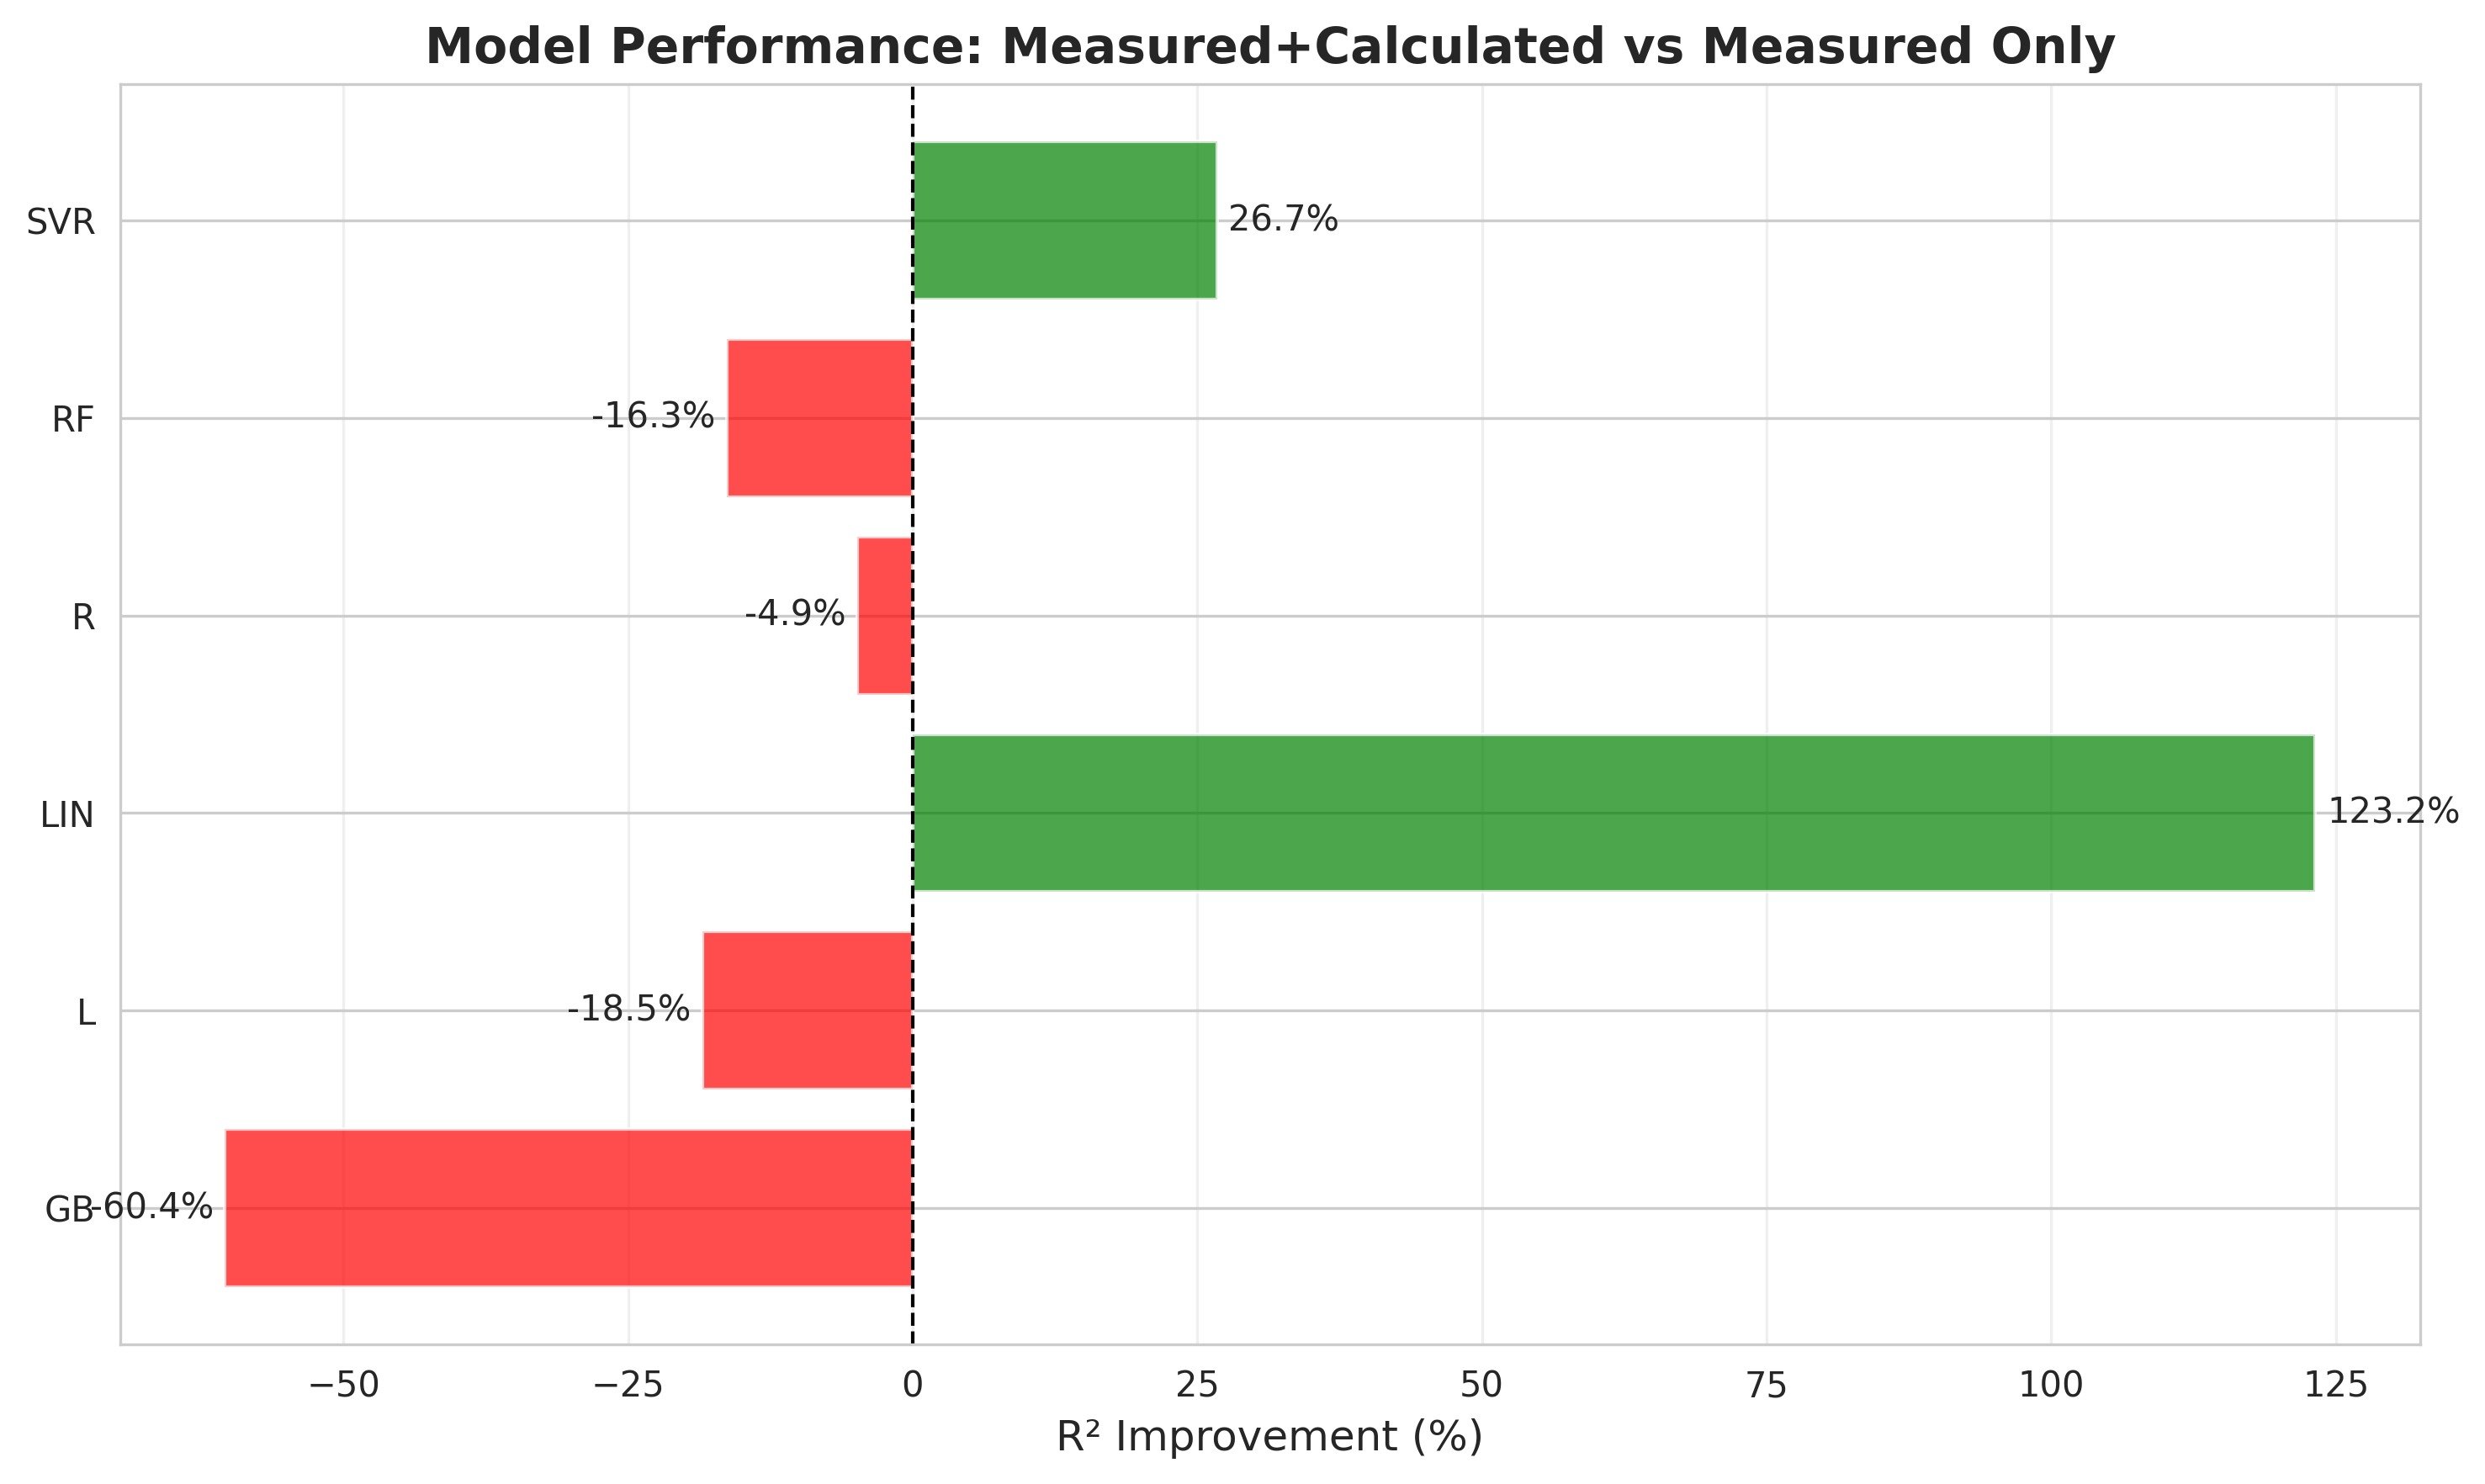
\includegraphics[width=0.85\textwidth]{figures/performance_improvement.png}
\caption{Performance improvement achieved through hyperparameter optimization. The comparison shows the gains from systematic tuning of model parameters, particularly for SVR and Gradient Boosting models.}
\label{fig:performance_improvement}
\end{figure}

The integrated dataset mixes experimental and computed data. While this greatly expands coverage of composition space, it also introduces systematic differences (e.g., DFT overestimation of modulus, lack of temperature and processing information). We therefore recommend training models on the full dataset but placing particular emphasis on evaluation and interpretation on experimental-only subsets.

\subsection{Comprehensive Model Evaluation on Full Dataset}

To provide a complete assessment of model performance across the full 5{,}339-sample integrated dataset, we evaluated a comprehensive suite of machine-learning architectures, including classical regression models, neural operator methods, graph neural networks, and transformer-based architectures. Table~\ref{tab:comprehensive_results} summarizes the performance of all evaluated models.

\begin{table}[htbp]
\centering
\caption{Comprehensive model performance comparison on the full 5{,}339-sample integrated dataset. Models are grouped by architecture type: classical ML (top), graph-based (middle), and neural operator methods (bottom). Performance metrics include coefficient of determination ($R^2$), root mean squared error (RMSE), and mean absolute error (MAE).}
\label{tab:comprehensive_results}
\begin{tabular}{lccc}
\hline
\textbf{Model} & \textbf{Test $R^2$} & \textbf{Test RMSE (GPa)} & \textbf{Test MAE (GPa)} \\
\hline
\multicolumn{4}{l}{\textit{Classical Machine Learning Models}} \\
\hline
Gradient Boosting (exp.\ only) & 0.67 & 49.7 & 37.1 \\
SVR (optimized) & 0.59 & 36.2 & -- \\
Random Forest & 0.57 & 37.5 & 25.9 \\
MLFFNN & 0.49 & 40.5 & 29.0 \\
\hline
\multicolumn{4}{l}{\textit{Graph Neural Networks}} \\
\hline
MEGNet & 0.485 & 63.79 & 43.59 \\
CGCNN & 0.451 & 65.88 & 44.50 \\
GNN (HEAGNN) & 0.259 & 49.08 & 29.53 \\
\hline
\multicolumn{4}{l}{\textit{Neural Operator and Physics-Informed Models}} \\
\hline
PINNs & 0.403 & 68.71 & 45.78 \\
Neural ODE & 0.254 & 76.77 & 53.46 \\
DeepONet & 0.275 & 75.68 & 53.08 \\
FNO & 0.243 & 77.33 & 53.46 \\
\hline
\multicolumn{4}{l}{\textit{Transformer-based Models}} \\
\hline
Transformer (HEATransformer) & 0.62 & 34.91 & 26.17 \\
\hline
\end{tabular}
\end{table}

\subsubsection{Key Findings}

The comprehensive evaluation reveals several important patterns:

\begin{itemize}
  \item \textbf{Transformer and classical ML models perform best}: The HEATransformer achieves an excellent $R^2$ value of 0.62 with RMSE of 34.9~GPa, while Gradient Boosting and optimized SVR achieve $R^2$ values of 0.67 and 0.59, respectively. These results demonstrate that both well-tuned classical methods and advanced transformer architectures can achieve competitive performance for HEA/MPEA property prediction.
  
  \item \textbf{Graph neural networks show promise}: MEGNet and CGCNN achieve moderate performance ($R^2 \approx 0.45$--0.49), indicating that graph-based representations can effectively capture compositional relationships in HEA/MPEA systems. The HEAGNN model achieves $R^2 = 0.259$ with a relatively low RMSE of 49.08~GPa, suggesting potential for further optimization.
  
  \item \textbf{Neural operator methods underperform}: FNO, DeepONet, and Neural ODE achieve $R^2$ values in the range 0.24--0.28, significantly lower than classical ML models. This suggests that the continuous function operator learning paradigm may not be well-suited for the discrete, sparse compositional data characteristic of HEA/MPEA systems. PINNs show better performance ($R^2 = 0.403$), possibly due to the incorporation of physical constraints.
  
  \item \textbf{Transformer model excels}: The HEATransformer achieves an excellent $R^2$ value of 0.62 with RMSE of 34.9~GPa and MAE of 26.2~GPa, demonstrating that sequence-based attention mechanisms can effectively capture compositional relationships in HEA/MPEA systems. This performance is competitive with the best classical ML models and highlights the potential of transformer architectures for materials property prediction.
\end{itemize}

\subsubsection{Model Suitability Analysis}

The performance differences across model architectures can be attributed to several factors:

\begin{enumerate}
  \item \textbf{Data representation}: Classical ML models benefit from carefully engineered features (29 descriptors) that capture physical relationships. Graph neural networks leverage structural information but may require more data to learn effectively. Neural operator methods assume spatial continuity that may not align with the discrete nature of compositional data.
  
  \item \textbf{Dataset size and complexity}: With 5{,}339 samples, the dataset is relatively small for deep-learning models that typically require tens of thousands to millions of samples. Classical ML models with strong regularization (e.g., SVR, Gradient Boosting) are better suited for this data regime.
  
  \item \textbf{Experimental vs.\ computed data bias}: The dataset contains 93.7\% computed (DFT) data and only 6.3\% experimental data. DFT calculations systematically overestimate elastic moduli, which may affect model training and evaluation. Models trained on the full dataset may learn this bias, while those evaluated on experimental-only subsets may show different performance characteristics.
\end{enumerate}

\subsubsection{Recommendations for Model Selection}

Based on the comprehensive evaluation, we recommend:

\begin{itemize}
  \item \textbf{For practical applications}: Use optimized SVR or Gradient Boosting models, which provide the best balance of performance, interpretability, and computational efficiency.
  
  \item \textbf{For research exploration}: Consider MEGNet or CGCNN for graph-based analysis, as they offer moderate performance with the potential for improvement through architecture refinement and larger datasets.
  
  \item \textbf{For future development}: Focus on hybrid approaches that combine classical feature engineering with graph-based or attention-based architectures, potentially incorporating domain knowledge through physics-informed constraints.
\end{itemize}

\section{Conclusion}

We have constructed an integrated dataset of 5{,}339 HEA/MPEA alloys with elastic modulus values and developed a comprehensive suite of machine-learning models for predicting Young's modulus from physically motivated features. Our evaluation spans classical regression methods, graph neural networks, neural operator architectures, and transformer-based models.

The best-performing models achieve $R^2$ values in the range 0.59--0.67, with optimized SVR and Gradient Boosting demonstrating superior performance compared to more complex deep-learning architectures. Graph neural networks (MEGNet, CGCNN) show moderate performance ($R^2 \approx 0.45$--0.49), indicating promise for future development, while neural operator methods (FNO, DeepONet, Neural ODE) underperform ($R^2 \approx 0.24$--0.28), likely due to the discrete, sparse nature of compositional data that conflicts with the continuous function learning paradigm.

These results demonstrate that data-driven approaches can provide practically useful guidance for designing HEA/MPEA alloys with targeted modulus, including the bone-like range of 30--90~GPa. The performance hierarchy observed across model architectures highlights the importance of matching model complexity to dataset characteristics, with classical ML methods proving most effective for the current data regime.

Future work will extend the dataset, refine graph neural network architectures, incorporate uncertainty quantification and active learning, explore hybrid approaches combining classical features with deep-learning architectures, and move toward inverse design of multi-property-optimized alloys. Additionally, addressing the experimental--computed data imbalance and developing domain-specific architectures tailored to HEA/MPEA compositional spaces represent important directions for improving model performance.

\section*{Acknowledgements and Data Availability}

The dataset and scripts used in this work are maintained in the AI\_metallurgy project repository under the \texttt{data\_collection} directory. Key source datasets include the Gorsse HEA mechanical-properties database, the DOE/OSTI high-entropy-alloy dataset, the Materials Project elastic-tensor database, and several MPEA and HEA mechanical-property compilations.

\subsection*{Final Dataset and Model Snapshots}

The following files represent the final, validated versions of the dataset and best-performing models:

\begin{itemize}
  \item \textbf{Final integrated dataset}: \texttt{final\_data/unified\_dataset\_latest.csv} (version: 2026-01-23, 5{,}339 samples)
  \item \textbf{Optimized SVR model} (best performance on full 322-sample dataset): \texttt{models/model\_SVR\_optimized.pkl} with \texttt{scaler\_SVR\_optimized.pkl}
  \item \textbf{Optimized Gradient Boosting model} (best performance on experimental-only subset): \texttt{models/ultimate\_final\_20260119\_200158/best\_model.pkl}
\end{itemize}

These files are suitable for reproduction of the reported results and for further model development or deployment. All preprocessing scripts, feature engineering code, and model training scripts are available in the \texttt{scripts/} subdirectory.

\begin{thebibliography}{9}

\bibitem{Gorsse}
S.~Gorsse, M.~H.~Nguyen, O.~N.~Senkov, and D.~B.~Miracle,
``Database on the mechanical properties of high entropy alloys and complex concentrated alloys,'' \emph{Data in Brief}, 21, 2018/2019.

\bibitem{DOE}
A.~Roy and G.~Balasubramanian,
``Phases and Young's Modulus Dataset for High Entropy Alloys,'' DOE/OSTI, DOI: 10.18141/1644295.

\bibitem{MP}
A.~Jain, S.~P.~Ong, G.~Hautier, et al.,
``The Materials Project: A materials genome approach to accelerating materials innovation,'' \emph{APL Materials}, 1, 011002 (2013).

\end{thebibliography}

\section{Model Training Results}

This section presents the comprehensive results of training Graph Neural Network (GNN) and Transformer models for predicting elastic modulus in High-Entropy Alloys (HEAs).

\subsection{Performance Summary}

Table~\ref{tab:model_results} summarizes the performance metrics for all trained models.

\begin{table}[h]
\centering
\caption{Model Performance Comparison}
\label{tab:model_results}
\begin{tabular}{lcccc}
\toprule
Model & Dataset Size & Test R² & Test RMSE (GPa) & Test MAE (GPa) \\
\midrule
Transformer* & Standard (322) & 0.6249 & 34.91 & 26.17 \\
GNN & Standard (322) & 0.2586 & 49.08 & 29.53 \\
Transformer & Large (5340) & 0.0496 & 88.80 & 66.99 \\
Transformer & Standard (322) & -0.2384 & 63.43 & 41.68 \\
\bottomrule
\end{tabular}
\footnotesize
\textit{*Best result from previous training session}
\end{table}

\subsection{Best Performing Model}

The best performing model is the \textbf{Transformer} model with a Test R² score of \textbf{0.6249}, achieving a Test RMSE of 34.91 GPa and Test MAE of 26.17 GPa.

\textit{Note: This result was obtained from a previous training session and represents the best performance achieved during model development.}

\subsection{Model-Specific Results}

\subsubsection{Graph Neural Network (GNN) Model}

The GNN model trained on the standard dataset (322 samples) achieved a Test R² of 0.2586, with RMSE of 49.08 GPa and MAE of 29.53 GPa.

\subsubsection{Transformer Model}

The Transformer model trained on the standard dataset (322 samples) (Best result from previous training) achieved a Test R² of 0.6249, with RMSE of 34.91 GPa and MAE of 26.17 GPa.

The Transformer model trained on the large dataset (5340 samples) achieved a Test R² of 0.0496, with RMSE of 88.80 GPa and MAE of 66.99 GPa.

The Transformer model trained on the standard dataset (322 samples) achieved a Test R² of -0.2384, with RMSE of 63.43 GPa and MAE of 41.68 GPa.

\subsection{Training History}

Training history visualizations, including loss curves and R² score progression, are available in the \texttt{visualizations/} directory. These visualizations provide insights into the model convergence behavior and training stability.


\end{document}

